% Options for packages loaded elsewhere
\PassOptionsToPackage{unicode}{hyperref}
\PassOptionsToPackage{hyphens}{url}
\PassOptionsToPackage{dvipsnames,svgnames,x11names}{xcolor}
%
\documentclass[
  11pt,
  a4paper,
  DIV=11,
  numbers=noendperiod]{scrartcl}

\usepackage{amsmath,amssymb}
\usepackage{iftex}
\ifPDFTeX
  \usepackage[T1]{fontenc}
  \usepackage[utf8]{inputenc}
  \usepackage{textcomp} % provide euro and other symbols
\else % if luatex or xetex
  \usepackage{unicode-math}
  \defaultfontfeatures{Scale=MatchLowercase}
  \defaultfontfeatures[\rmfamily]{Ligatures=TeX,Scale=1}
\fi
\usepackage{lmodern}
\ifPDFTeX\else  
    % xetex/luatex font selection
\fi
% Use upquote if available, for straight quotes in verbatim environments
\IfFileExists{upquote.sty}{\usepackage{upquote}}{}
\IfFileExists{microtype.sty}{% use microtype if available
  \usepackage[]{microtype}
  \UseMicrotypeSet[protrusion]{basicmath} % disable protrusion for tt fonts
}{}
\makeatletter
\@ifundefined{KOMAClassName}{% if non-KOMA class
  \IfFileExists{parskip.sty}{%
    \usepackage{parskip}
  }{% else
    \setlength{\parindent}{0pt}
    \setlength{\parskip}{6pt plus 2pt minus 1pt}}
}{% if KOMA class
  \KOMAoptions{parskip=half}}
\makeatother
\usepackage{xcolor}
\usepackage[margin=0.8in]{geometry}
\setlength{\emergencystretch}{3em} % prevent overfull lines
\setcounter{secnumdepth}{3}
% Make \paragraph and \subparagraph free-standing
\makeatletter
\ifx\paragraph\undefined\else
  \let\oldparagraph\paragraph
  \renewcommand{\paragraph}{
    \@ifstar
      \xxxParagraphStar
      \xxxParagraphNoStar
  }
  \newcommand{\xxxParagraphStar}[1]{\oldparagraph*{#1}\mbox{}}
  \newcommand{\xxxParagraphNoStar}[1]{\oldparagraph{#1}\mbox{}}
\fi
\ifx\subparagraph\undefined\else
  \let\oldsubparagraph\subparagraph
  \renewcommand{\subparagraph}{
    \@ifstar
      \xxxSubParagraphStar
      \xxxSubParagraphNoStar
  }
  \newcommand{\xxxSubParagraphStar}[1]{\oldsubparagraph*{#1}\mbox{}}
  \newcommand{\xxxSubParagraphNoStar}[1]{\oldsubparagraph{#1}\mbox{}}
\fi
\makeatother

\usepackage{color}
\usepackage{fancyvrb}
\newcommand{\VerbBar}{|}
\newcommand{\VERB}{\Verb[commandchars=\\\{\}]}
\DefineVerbatimEnvironment{Highlighting}{Verbatim}{commandchars=\\\{\}}
% Add ',fontsize=\small' for more characters per line
\usepackage{framed}
\definecolor{shadecolor}{RGB}{241,243,245}
\newenvironment{Shaded}{\begin{snugshade}}{\end{snugshade}}
\newcommand{\AlertTok}[1]{\textcolor[rgb]{0.68,0.00,0.00}{#1}}
\newcommand{\AnnotationTok}[1]{\textcolor[rgb]{0.37,0.37,0.37}{#1}}
\newcommand{\AttributeTok}[1]{\textcolor[rgb]{0.40,0.45,0.13}{#1}}
\newcommand{\BaseNTok}[1]{\textcolor[rgb]{0.68,0.00,0.00}{#1}}
\newcommand{\BuiltInTok}[1]{\textcolor[rgb]{0.00,0.23,0.31}{#1}}
\newcommand{\CharTok}[1]{\textcolor[rgb]{0.13,0.47,0.30}{#1}}
\newcommand{\CommentTok}[1]{\textcolor[rgb]{0.37,0.37,0.37}{#1}}
\newcommand{\CommentVarTok}[1]{\textcolor[rgb]{0.37,0.37,0.37}{\textit{#1}}}
\newcommand{\ConstantTok}[1]{\textcolor[rgb]{0.56,0.35,0.01}{#1}}
\newcommand{\ControlFlowTok}[1]{\textcolor[rgb]{0.00,0.23,0.31}{\textbf{#1}}}
\newcommand{\DataTypeTok}[1]{\textcolor[rgb]{0.68,0.00,0.00}{#1}}
\newcommand{\DecValTok}[1]{\textcolor[rgb]{0.68,0.00,0.00}{#1}}
\newcommand{\DocumentationTok}[1]{\textcolor[rgb]{0.37,0.37,0.37}{\textit{#1}}}
\newcommand{\ErrorTok}[1]{\textcolor[rgb]{0.68,0.00,0.00}{#1}}
\newcommand{\ExtensionTok}[1]{\textcolor[rgb]{0.00,0.23,0.31}{#1}}
\newcommand{\FloatTok}[1]{\textcolor[rgb]{0.68,0.00,0.00}{#1}}
\newcommand{\FunctionTok}[1]{\textcolor[rgb]{0.28,0.35,0.67}{#1}}
\newcommand{\ImportTok}[1]{\textcolor[rgb]{0.00,0.46,0.62}{#1}}
\newcommand{\InformationTok}[1]{\textcolor[rgb]{0.37,0.37,0.37}{#1}}
\newcommand{\KeywordTok}[1]{\textcolor[rgb]{0.00,0.23,0.31}{\textbf{#1}}}
\newcommand{\NormalTok}[1]{\textcolor[rgb]{0.00,0.23,0.31}{#1}}
\newcommand{\OperatorTok}[1]{\textcolor[rgb]{0.37,0.37,0.37}{#1}}
\newcommand{\OtherTok}[1]{\textcolor[rgb]{0.00,0.23,0.31}{#1}}
\newcommand{\PreprocessorTok}[1]{\textcolor[rgb]{0.68,0.00,0.00}{#1}}
\newcommand{\RegionMarkerTok}[1]{\textcolor[rgb]{0.00,0.23,0.31}{#1}}
\newcommand{\SpecialCharTok}[1]{\textcolor[rgb]{0.37,0.37,0.37}{#1}}
\newcommand{\SpecialStringTok}[1]{\textcolor[rgb]{0.13,0.47,0.30}{#1}}
\newcommand{\StringTok}[1]{\textcolor[rgb]{0.13,0.47,0.30}{#1}}
\newcommand{\VariableTok}[1]{\textcolor[rgb]{0.07,0.07,0.07}{#1}}
\newcommand{\VerbatimStringTok}[1]{\textcolor[rgb]{0.13,0.47,0.30}{#1}}
\newcommand{\WarningTok}[1]{\textcolor[rgb]{0.37,0.37,0.37}{\textit{#1}}}

\providecommand{\tightlist}{%
  \setlength{\itemsep}{0pt}\setlength{\parskip}{0pt}}\usepackage{longtable,booktabs,array}
\usepackage{calc} % for calculating minipage widths
% Correct order of tables after \paragraph or \subparagraph
\usepackage{etoolbox}
\makeatletter
\patchcmd\longtable{\par}{\if@noskipsec\mbox{}\fi\par}{}{}
\makeatother
% Allow footnotes in longtable head/foot
\IfFileExists{footnotehyper.sty}{\usepackage{footnotehyper}}{\usepackage{footnote}}
\makesavenoteenv{longtable}
\usepackage{graphicx}
\makeatletter
\newsavebox\pandoc@box
\newcommand*\pandocbounded[1]{% scales image to fit in text height/width
  \sbox\pandoc@box{#1}%
  \Gscale@div\@tempa{\textheight}{\dimexpr\ht\pandoc@box+\dp\pandoc@box\relax}%
  \Gscale@div\@tempb{\linewidth}{\wd\pandoc@box}%
  \ifdim\@tempb\p@<\@tempa\p@\let\@tempa\@tempb\fi% select the smaller of both
  \ifdim\@tempa\p@<\p@\scalebox{\@tempa}{\usebox\pandoc@box}%
  \else\usebox{\pandoc@box}%
  \fi%
}
% Set default figure placement to htbp
\def\fps@figure{htbp}
\makeatother

% tex header includes


%\usepackage[T1]{fontenc}     % Ensures proper character encoding
%\usepackage{textcomp}        % Provides additional symbols
%\usepackage{newtxtext}       % Equivalent to Stix Two Text for text
%\usepackage{stix2}       % GPT says load here  Equivalent to Stix Two Math for math

\usepackage{amsmath}
\usepackage{amssymb}         % If needed

\usepackage{multirow}
\usepackage{url}
\usepackage{tikz}
\usepackage{color}

\usetikzlibrary{arrows,calc,positioning,shadows.blur,decorations.pathreplacing}
\usetikzlibrary{automata}
\usetikzlibrary{fit}
\usetikzlibrary{snakes}
\usetikzlibrary{intersections}
\usetikzlibrary{decorations.markings,decorations.text, decorations.pathmorphing,decorations.shapes}
\usetikzlibrary{decorations.fractals,decorations.footprints}
\usetikzlibrary{graphs}
\usetikzlibrary{matrix}
\usetikzlibrary{shapes.geometric}
\usetikzlibrary{mindmap, shadows}
\usetikzlibrary{backgrounds}
\usetikzlibrary{cd}

\newcommand{\grtspacer}{\vphantom{lp}}
\KOMAoption{captions}{tableheading}
\makeatletter
\@ifpackageloaded{caption}{}{\usepackage{caption}}
\AtBeginDocument{%
\ifdefined\contentsname
  \renewcommand*\contentsname{Table of contents}
\else
  \newcommand\contentsname{Table of contents}
\fi
\ifdefined\listfigurename
  \renewcommand*\listfigurename{List of Figures}
\else
  \newcommand\listfigurename{List of Figures}
\fi
\ifdefined\listtablename
  \renewcommand*\listtablename{List of Tables}
\else
  \newcommand\listtablename{List of Tables}
\fi
\ifdefined\figurename
  \renewcommand*\figurename{Figure}
\else
  \newcommand\figurename{Figure}
\fi
\ifdefined\tablename
  \renewcommand*\tablename{Table}
\else
  \newcommand\tablename{Table}
\fi
}
\@ifpackageloaded{float}{}{\usepackage{float}}
\floatstyle{ruled}
\@ifundefined{c@chapter}{\newfloat{codelisting}{h}{lop}}{\newfloat{codelisting}{h}{lop}[chapter]}
\floatname{codelisting}{Listing}
\newcommand*\listoflistings{\listof{codelisting}{List of Listings}}
\makeatother
\makeatletter
\makeatother
\makeatletter
\@ifpackageloaded{caption}{}{\usepackage{caption}}
\@ifpackageloaded{subcaption}{}{\usepackage{subcaption}}
\makeatother

\usepackage{bookmark}

\IfFileExists{xurl.sty}{\usepackage{xurl}}{} % add URL line breaks if available
\urlstyle{same} % disable monospaced font for URLs
\hypersetup{
  pdftitle={All Tables Test - New TestDFGenerator test\_suite},
  pdfauthor={Stephen J. Mildenhall},
  colorlinks=true,
  linkcolor={blue},
  filecolor={Maroon},
  citecolor={Blue},
  urlcolor={Blue},
  pdfcreator={LaTeX via pandoc}}


\title{All Tables Test - New TestDFGenerator test\_suite}
\author{Stephen J. Mildenhall}
\date{2025-03-14}

\begin{document}
\maketitle


\phantomsection\label{setup}
\begin{Shaded}
\begin{Highlighting}[]
\ImportTok{from}\NormalTok{ IPython.display }\ImportTok{import}\NormalTok{ HTML, display}
\ImportTok{import}\NormalTok{ matplotlib }\ImportTok{as}\NormalTok{ mpl}
\ImportTok{import}\NormalTok{ matplotlib.dates }\ImportTok{as}\NormalTok{ mdates}
\ImportTok{import}\NormalTok{ matplotlib.pyplot }\ImportTok{as}\NormalTok{ plt}
\ImportTok{import}\NormalTok{ numpy }\ImportTok{as}\NormalTok{ np}
\ImportTok{import}\NormalTok{ pandas }\ImportTok{as}\NormalTok{ pd}

\ImportTok{import}\NormalTok{ greater\_tables }\ImportTok{as}\NormalTok{ gter}
\ImportTok{import}\NormalTok{ greater\_tables.utilities }\ImportTok{as}\NormalTok{ gtu}
\ImportTok{from}\NormalTok{ greater\_tables }\ImportTok{import}\NormalTok{ GT, sGT}
\NormalTok{gter.logger.setLevel(gter.logging.WARNING)}
\end{Highlighting}
\end{Shaded}

\ldots code build completed.

\section{A Hard-Rules table}\label{a-hard-rules-table}

Second level index has mixed types. Range of magnitudes. Picking out
years.

\begin{Shaded}
\begin{Highlighting}[]
\NormalTok{level\_1 }\OperatorTok{=}\NormalTok{ [}\StringTok{"A"}\NormalTok{, }\StringTok{"A"}\NormalTok{, }\StringTok{"B"}\NormalTok{, }\StringTok{"B"}\NormalTok{, }\StringTok{\textquotesingle{}C\textquotesingle{}}\NormalTok{]}
\NormalTok{level\_2 }\OperatorTok{=}\NormalTok{ [}\StringTok{\textquotesingle{}Int\textquotesingle{}}\NormalTok{, }\StringTok{\textquotesingle{}Float\textquotesingle{}}\NormalTok{, }\StringTok{\textquotesingle{}Float\textquotesingle{}}\NormalTok{, }\DecValTok{3}\NormalTok{, }\StringTok{\textquotesingle{}Longer Text\textquotesingle{}}\NormalTok{]}

\NormalTok{multi\_index }\OperatorTok{=}\NormalTok{ pd.MultiIndex.from\_arrays([level\_1, level\_2],}
\NormalTok{        names}\OperatorTok{=}\NormalTok{[}\StringTok{"Level 1"}\NormalTok{, }\StringTok{"Level 2"}\NormalTok{])}
\NormalTok{start }\OperatorTok{=}\NormalTok{ pd.Timestamp.today().normalize()  }\CommentTok{\# Today\textquotesingle{}s date, normalized to midnight}
\NormalTok{end }\OperatorTok{=}\NormalTok{ pd.Timestamp(}\SpecialStringTok{f"}\SpecialCharTok{\{}\NormalTok{start}\SpecialCharTok{.}\NormalTok{year}\SpecialCharTok{\}}\SpecialStringTok{{-}12{-}31"}\NormalTok{)  }\CommentTok{\# End of the year}

\NormalTok{hard }\OperatorTok{=}\NormalTok{ pd.DataFrame(}
\NormalTok{\{}\StringTok{\textquotesingle{}years!\textquotesingle{}}\NormalTok{: np.arange(}\DecValTok{2000}\NormalTok{, }\DecValTok{2025}\NormalTok{, dtype}\OperatorTok{=}\BuiltInTok{int}\NormalTok{),}
\StringTok{\textquotesingle{}a\textquotesingle{}}\NormalTok{: np.array(np.}\BuiltInTok{round}\NormalTok{(np.linspace(}\OperatorTok{{-}}\DecValTok{100000}\NormalTok{, }\DecValTok{100000}\NormalTok{, }\DecValTok{25}\NormalTok{), }\DecValTok{0}\NormalTok{), dtype}\OperatorTok{=}\BuiltInTok{int}\NormalTok{),}
\StringTok{\textquotesingle{}b\textquotesingle{}}\NormalTok{: }\FloatTok{9.3} \OperatorTok{**}\NormalTok{ np.linspace(}\OperatorTok{{-}}\DecValTok{12}\NormalTok{, }\DecValTok{12}\NormalTok{, }\DecValTok{25}\NormalTok{),}
\StringTok{\textquotesingle{}c\textquotesingle{}}\NormalTok{: np.linspace(}\OperatorTok{{-}}\DecValTok{1601}\NormalTok{, }\DecValTok{4000}\NormalTok{, }\DecValTok{25}\NormalTok{),}
\StringTok{\textquotesingle{}d\textquotesingle{}}\NormalTok{: pd.date\_range(start}\OperatorTok{=}\NormalTok{start, end}\OperatorTok{=}\NormalTok{end, periods}\OperatorTok{=}\DecValTok{25}\NormalTok{),}
\StringTok{\textquotesingle{}e\textquotesingle{}}\NormalTok{: (}\StringTok{\textquotesingle{}once upon a time, risk is hard to define, not in Kansas anymore, \textquotesingle{}}
        \StringTok{\textquotesingle{}neutrinos are hard to detect,  \textquotesingle{}}
        \StringTok{\textquotesingle{}Adam Smith is the father of economics\textquotesingle{}}\NormalTok{.split(}\StringTok{\textquotesingle{},\textquotesingle{}}\NormalTok{) }\OperatorTok{*} \DecValTok{5}\NormalTok{)}
\NormalTok{\}).set\_index(}\StringTok{\textquotesingle{}years!\textquotesingle{}}\NormalTok{)}
\CommentTok{\# hard = hard.head()}
\NormalTok{hard.columns }\OperatorTok{=}\NormalTok{ multi\_index}
\NormalTok{hard}
\end{Highlighting}
\end{Shaded}

\begin{longtable}[]{@{}llllll@{}}

\caption{\label{tbl-hard-rules}Default display output (Quarto generated
caption)}

\tabularnewline

\toprule\noalign{}
Level 1 & \multicolumn{2}{l}{%
A} & \multicolumn{2}{l}{%
B} & C \\
Level 2 & Int & Float & Float & 3 & Longer Text \\
years! & & & & & \\
\midrule\noalign{}
\endhead
\bottomrule\noalign{}
\endlastfoot
2000 & -100000 & 2.388937e-12 & -1601.000 & 2025-03-14 00:00:00 & once
upon a time \\
2001 & -91667 & 2.221711e-11 & -1367.625 & 2025-03-26 04:00:00 & risk is
hard to define \\
2002 & -83333 & 2.066191e-10 & -1134.250 & 2025-04-07 08:00:00 & not in
Kansas anymore \\
2003 & -75000 & 1.921558e-09 & -900.875 & 2025-04-19 12:00:00 &
neutrinos are hard to detect \\
2004 & -66667 & 1.787049e-08 & -667.500 & 2025-05-01 16:00:00 & Adam
Smith is the father of economics \\
2005 & -58333 & 1.661955e-07 & -434.125 & 2025-05-13 20:00:00 & once
upon a time \\
2006 & -50000 & 1.545619e-06 & -200.750 & 2025-05-26 00:00:00 & risk is
hard to define \\
2007 & -41667 & 1.437425e-05 & 32.625 & 2025-06-07 04:00:00 & not in
Kansas anymore \\
2008 & -33333 & 1.336805e-04 & 266.000 & 2025-06-19 08:00:00 & neutrinos
are hard to detect \\
2009 & -25000 & 1.243229e-03 & 499.375 & 2025-07-01 12:00:00 & Adam
Smith is the father of economics \\
2010 & -16667 & 1.156203e-02 & 732.750 & 2025-07-13 16:00:00 & once upon
a time \\
2011 & -8333 & 1.075269e-01 & 966.125 & 2025-07-25 20:00:00 & risk is
hard to define \\
2012 & 0 & 1.000000e+00 & 1199.500 & 2025-08-07 00:00:00 & not in Kansas
anymore \\
2013 & 8333 & 9.300000e+00 & 1432.875 & 2025-08-19 04:00:00 & neutrinos
are hard to detect \\
2014 & 16667 & 8.649000e+01 & 1666.250 & 2025-08-31 08:00:00 & Adam
Smith is the father of economics \\
2015 & 25000 & 8.043570e+02 & 1899.625 & 2025-09-12 12:00:00 & once upon
a time \\
2016 & 33333 & 7.480520e+03 & 2133.000 & 2025-09-24 16:00:00 & risk is
hard to define \\
2017 & 41667 & 6.956884e+04 & 2366.375 & 2025-10-06 20:00:00 & not in
Kansas anymore \\
2018 & 50000 & 6.469902e+05 & 2599.750 & 2025-10-19 00:00:00 & neutrinos
are hard to detect \\
2019 & 58333 & 6.017009e+06 & 2833.125 & 2025-10-31 04:00:00 & Adam
Smith is the father of economics \\
2020 & 66667 & 5.595818e+07 & 3066.500 & 2025-11-12 08:00:00 & once upon
a time \\
2021 & 75000 & 5.204111e+08 & 3299.875 & 2025-11-24 12:00:00 & risk is
hard to define \\
2022 & 83333 & 4.839823e+09 & 3533.250 & 2025-12-06 16:00:00 & not in
Kansas anymore \\
2023 & 91667 & 4.501035e+10 & 3766.625 & 2025-12-18 20:00:00 & neutrinos
are hard to detect \\
2024 & 100000 & 4.185963e+11 & 4000.000 & 2025-12-31 00:00:00 & Adam
Smith is the father of economics \\

\end{longtable}

Table~\ref{tbl-hard-rules} shows the default output and
Table~\ref{tbl-hard-rules-2} the \texttt{sGT} format output.

\begin{Shaded}
\begin{Highlighting}[]
\NormalTok{sGT(hard, }\StringTok{\textquotesingle{}A table with varied columns.\textquotesingle{}}\NormalTok{)}
\end{Highlighting}
\end{Shaded}

\begin{table}

\caption{\label{tbl-hard-rules-2}Greater Tables output (Quarto generated
caption)}

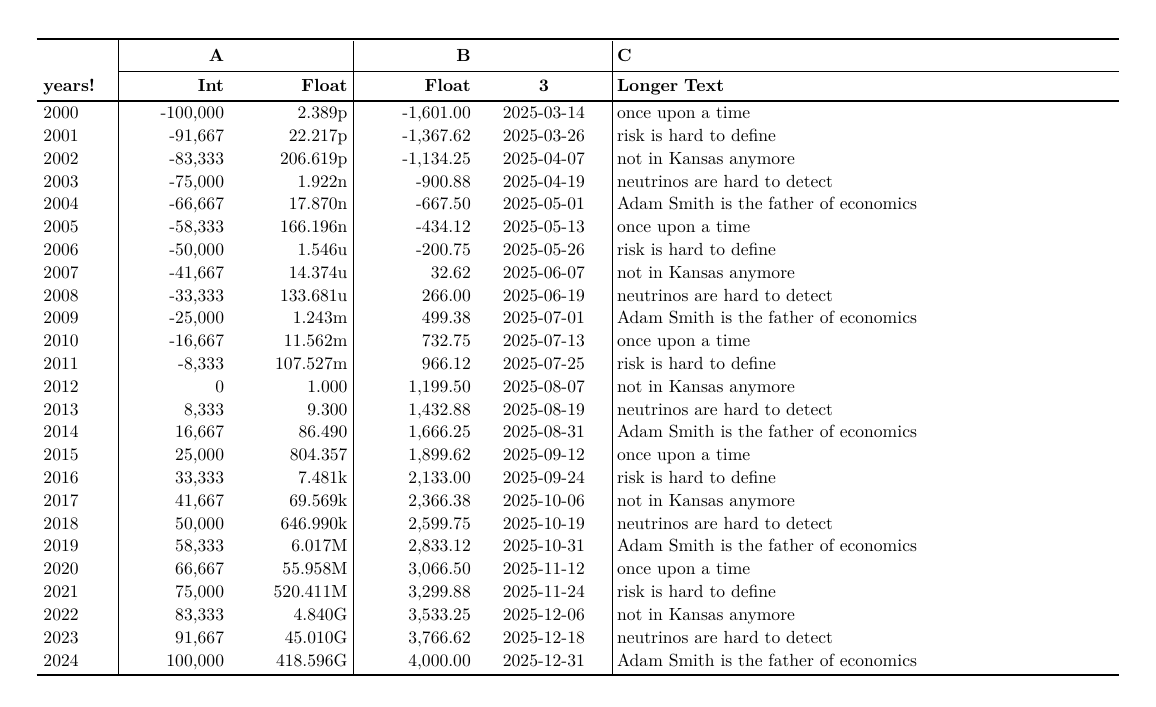
\begin{tikzpicture}[
    auto,
    transform shape,
    nosep/.style={inner sep=0},
    table/.style={
        matrix of nodes,
        row sep=0.125em,
        column sep=0.375em,
        nodes in empty cells,
        nodes={rectangle, scale=0.635, text badly ragged },
    row 1/.style={nodes={text=black, anchor=north, inner ysep=0, text height=0, text depth=0}},
    row 2/.style={nodes={text=black, anchor=south, inner ysep=.2em, minimum height=1.3em, font=\bfseries}},
    row 3/.style={nodes={text=black, anchor=south, inner ysep=.2em, minimum height=1.3em, font=\bfseries}},
    column  1/.style={nodes={align=left  }, text height=0.9em, text depth=0.2em, inner xsep=0.375em, inner ysep=0, text width=3.60em},
    column  2/.style={nodes={align=right }, nosep, text width=5.71em},
    column  3/.style={nodes={align=right }, nosep, text width=6.43em},
    column  4/.style={nodes={align=right }, nosep, text width=6.43em},
    column  5/.style={nodes={align=center}, nosep, text width=7.14em},
    column  6/.style={nodes={align=left  }, nosep, text width=27.85em},
    column  7/.style={text height=0.9em, text depth=0.2em, nosep, text width=0em}   }]
\matrix (T4JQAJ5YI3QMU) [table, ampersand replacement=\&]{
      \&          \&           \&           \&            \&                                         \& \\
 \grtspacer \& A\grtspacer \& \grtspacer \& B\grtspacer \& \grtspacer \& C\grtspacer                             \& \\
 years!\grtspacer \& Int\grtspacer \& Float\grtspacer \& Float\grtspacer \& 3\grtspacer \& Longer Text\grtspacer                   \& \\
 2000 \& -100,000 \&    2.389p \& -1,601.00 \& 2025-03-14 \& once upon a time                        \& \\
 2001 \&  -91,667 \&   22.217p \& -1,367.62 \& 2025-03-26 \&  risk is hard to define                 \& \\
 2002 \&  -83,333 \&  206.619p \& -1,134.25 \& 2025-04-07 \&  not in Kansas anymore                  \& \\
 2003 \&  -75,000 \&    1.922n \&   -900.88 \& 2025-04-19 \&  neutrinos are hard to detect           \& \\
 2004 \&  -66,667 \&   17.870n \&   -667.50 \& 2025-05-01 \&   Adam Smith is the father of economics \& \\
 2005 \&  -58,333 \&  166.196n \&   -434.12 \& 2025-05-13 \& once upon a time                        \& \\
 2006 \&  -50,000 \&    1.546u \&   -200.75 \& 2025-05-26 \&  risk is hard to define                 \& \\
 2007 \&  -41,667 \&   14.374u \&     32.62 \& 2025-06-07 \&  not in Kansas anymore                  \& \\
 2008 \&  -33,333 \&  133.681u \&    266.00 \& 2025-06-19 \&  neutrinos are hard to detect           \& \\
 2009 \&  -25,000 \&    1.243m \&    499.38 \& 2025-07-01 \&   Adam Smith is the father of economics \& \\
 2010 \&  -16,667 \&   11.562m \&    732.75 \& 2025-07-13 \& once upon a time                        \& \\
 2011 \&   -8,333 \&  107.527m \&    966.12 \& 2025-07-25 \&  risk is hard to define                 \& \\
 2012 \&        0 \&     1.000 \&  1,199.50 \& 2025-08-07 \&  not in Kansas anymore                  \& \\
 2013 \&    8,333 \&     9.300 \&  1,432.88 \& 2025-08-19 \&  neutrinos are hard to detect           \& \\
 2014 \&   16,667 \&    86.490 \&  1,666.25 \& 2025-08-31 \&   Adam Smith is the father of economics \& \\
 2015 \&   25,000 \&   804.357 \&  1,899.62 \& 2025-09-12 \& once upon a time                        \& \\
 2016 \&   33,333 \&    7.481k \&  2,133.00 \& 2025-09-24 \&  risk is hard to define                 \& \\
 2017 \&   41,667 \&   69.569k \&  2,366.38 \& 2025-10-06 \&  not in Kansas anymore                  \& \\
 2018 \&   50,000 \&  646.990k \&  2,599.75 \& 2025-10-19 \&  neutrinos are hard to detect           \& \\
 2019 \&   58,333 \&    6.017M \&  2,833.12 \& 2025-10-31 \&   Adam Smith is the father of economics \& \\
 2020 \&   66,667 \&   55.958M \&  3,066.50 \& 2025-11-12 \& once upon a time                        \& \\
 2021 \&   75,000 \&  520.411M \&  3,299.88 \& 2025-11-24 \&  risk is hard to define                 \& \\
 2022 \&   83,333 \&    4.840G \&  3,533.25 \& 2025-12-06 \&  not in Kansas anymore                  \& \\
 2023 \&   91,667 \&   45.010G \&  3,766.62 \& 2025-12-18 \&  neutrinos are hard to detect           \& \\
 2024 \&  100,000 \&  418.596G \&  4,000.00 \& 2025-12-31 \&   Adam Smith is the father of economics \& \\
};

\path[draw, thick] (T4JQAJ5YI3QMU-1-1.south west)  -- (T4JQAJ5YI3QMU-1-7.south east);
\path[draw, semithick] ([yshift=-0.0625em]T4JQAJ5YI3QMU-3-1.south west)  -- ([yshift=-0.0625em]T4JQAJ5YI3QMU-3-7.south east);
\path[draw, thick] ([yshift=-0.3125em]T4JQAJ5YI3QMU-28-1.base west)  -- ([yshift=-0.3125em]T4JQAJ5YI3QMU-28-7.base east);
\path[draw, very thin] ([xshift=-0.1875em, yshift=-0.0625em]T4JQAJ5YI3QMU-2-2.south west)  -- ([yshift=-0.0625em]T4JQAJ5YI3QMU-2-7.south east);
\path[draw, very thin] ([xshift=-0.1875em]T4JQAJ5YI3QMU-1-2.south west)  -- ([yshift=-0.3125em, xshift=-0.1875em]T4JQAJ5YI3QMU-28-2.base west);
\path[draw, ultra thin] ([xshift=0.1875em, yshift=-0.0625em]T4JQAJ5YI3QMU-1-3.south east)  -- ([yshift=-0.3125em, xshift=0.1875em]T4JQAJ5YI3QMU-28-3.base east);
\path[draw, ultra thin] ([xshift=0.1875em, yshift=-0.0625em]T4JQAJ5YI3QMU-1-5.south east)  -- ([yshift=-0.3125em, xshift=0.1875em]T4JQAJ5YI3QMU-28-5.base east);



\end{tikzpicture}

\end{table}%

Here are some alternatives:

\begin{itemize}
\tightlist
\item
  Table~\ref{tbl-hard-rules-3a} hrules no vrules
\item
  Table~\ref{tbl-hard-rules-3b} change date and integer formats and
\item
  Table~\ref{tbl-hard-rules-3c} change padding and debug mode.
\end{itemize}

\begin{Shaded}
\begin{Highlighting}[]
\InformationTok{\textasciigrave{}\textasciigrave{}\textasciigrave{}\{python\}}
\InformationTok{\#| label: tbl{-}hard{-}rules{-}3a}
\InformationTok{\#| tbl{-}cap: No V rules but hrules (Quarto generated caption)}
\InformationTok{display(sGT(hard.sample(5).sort\_index(),}
\InformationTok{        caption=\textquotesingle{}GT caption No v rules, but h rules\textquotesingle{},}
\InformationTok{        vrule\_widths=(0,0,0),}
\InformationTok{        hrule\_widths=(1,0,0)))}
\InformationTok{\textasciigrave{}\textasciigrave{}\textasciigrave{}}
\end{Highlighting}
\end{Shaded}

\begin{table}

\caption{\label{tbl-hard-rules-3a}No V rules but hrules (Quarto
generated caption)}

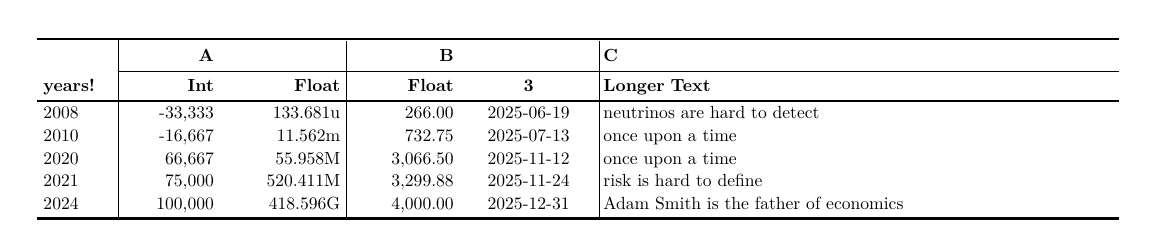
\begin{tikzpicture}[
    auto,
    transform shape,
    nosep/.style={inner sep=0},
    table/.style={
        matrix of nodes,
        row sep=0.125em,
        column sep=0.375em,
        nodes in empty cells,
        nodes={rectangle, scale=0.635, text badly ragged },
    row 1/.style={nodes={text=black, anchor=north, inner ysep=0, text height=0, text depth=0}},
    row 2/.style={nodes={text=black, anchor=south, inner ysep=.2em, minimum height=1.3em, font=\bfseries}},
    row 3/.style={nodes={text=black, anchor=south, inner ysep=.2em, minimum height=1.3em, font=\bfseries}},
    column  1/.style={nodes={align=left  }, text height=0.9em, text depth=0.2em, inner xsep=0.375em, inner ysep=0, text width=3.60em},
    column  2/.style={nodes={align=right }, nosep, text width=5.13em},
    column  3/.style={nodes={align=right }, nosep, text width=6.60em},
    column  4/.style={nodes={align=right }, nosep, text width=5.87em},
    column  5/.style={nodes={align=center}, nosep, text width=7.34em},
    column  6/.style={nodes={align=left  }, nosep, text width=28.61em},
    column  7/.style={text height=0.9em, text depth=0.2em, nosep, text width=0em}   }]
\matrix (TDYK7WPLIAE7W) [table, ampersand replacement=\&]{
      \&         \&           \&          \&            \&                                         \& \\
 \grtspacer \& A\grtspacer \& \grtspacer \& B\grtspacer \& \grtspacer \& C\grtspacer                             \& \\
 years!\grtspacer \& Int\grtspacer \& Float\grtspacer \& Float\grtspacer \& 3\grtspacer \& Longer Text\grtspacer                   \& \\
 2008 \& -33,333 \&  133.681u \&   266.00 \& 2025-06-19 \&  neutrinos are hard to detect           \& \\
 2010 \& -16,667 \&   11.562m \&   732.75 \& 2025-07-13 \& once upon a time                        \& \\
 2020 \&  66,667 \&   55.958M \& 3,066.50 \& 2025-11-12 \& once upon a time                        \& \\
 2021 \&  75,000 \&  520.411M \& 3,299.88 \& 2025-11-24 \&  risk is hard to define                 \& \\
 2024 \& 100,000 \&  418.596G \& 4,000.00 \& 2025-12-31 \&   Adam Smith is the father of economics \& \\
};

\path[draw, thick] (TDYK7WPLIAE7W-1-1.south west)  -- (TDYK7WPLIAE7W-1-7.south east);
\path[draw, semithick] ([yshift=-0.0625em]TDYK7WPLIAE7W-3-1.south west)  -- ([yshift=-0.0625em]TDYK7WPLIAE7W-3-7.south east);
\path[draw, thick] ([yshift=-0.3125em]TDYK7WPLIAE7W-8-1.base west)  -- ([yshift=-0.3125em]TDYK7WPLIAE7W-8-7.base east);
\path[draw, very thin] ([xshift=-0.1875em, yshift=-0.0625em]TDYK7WPLIAE7W-2-2.south west)  -- ([yshift=-0.0625em]TDYK7WPLIAE7W-2-7.south east);
\path[draw, very thin] ([xshift=-0.1875em]TDYK7WPLIAE7W-1-2.south west)  -- ([yshift=-0.3125em, xshift=-0.1875em]TDYK7WPLIAE7W-8-2.base west);
\path[draw, ultra thin] ([xshift=0.1875em, yshift=-0.0625em]TDYK7WPLIAE7W-1-3.south east)  -- ([yshift=-0.3125em, xshift=0.1875em]TDYK7WPLIAE7W-8-3.base east);
\path[draw, ultra thin] ([xshift=0.1875em, yshift=-0.0625em]TDYK7WPLIAE7W-1-5.south east)  -- ([yshift=-0.3125em, xshift=0.1875em]TDYK7WPLIAE7W-8-5.base east);



\end{tikzpicture}

\end{table}%

\begin{Shaded}
\begin{Highlighting}[]
\InformationTok{\textasciigrave{}\textasciigrave{}\textasciigrave{}\{python\}}
\InformationTok{\#| label: tbl{-}hard{-}rules{-}3b}
\InformationTok{\#| tbl{-}cap: Change date and integer formats  (Quarto generated caption)}
\InformationTok{display(sGT(hard.sample(5).sort\_index(),}
\InformationTok{        caption=\textquotesingle{}Change default date and integer formats\textquotesingle{},}
\InformationTok{        default\_date\_str=\textquotesingle{}\%m{-}\%d\textquotesingle{}, default\_integer\_str=\textquotesingle{}[\{x:d\}]\textquotesingle{}))}
\InformationTok{\textasciigrave{}\textasciigrave{}\textasciigrave{}}
\end{Highlighting}
\end{Shaded}

\begin{table}

\caption{\label{tbl-hard-rules-3b}Change date and integer formats
(Quarto generated caption)}

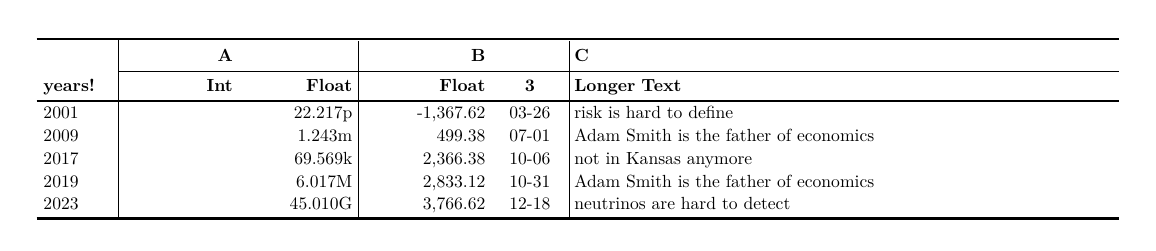
\begin{tikzpicture}[
    auto,
    transform shape,
    nosep/.style={inner sep=0},
    table/.style={
        matrix of nodes,
        row sep=0.125em,
        column sep=0.375em,
        nodes in empty cells,
        nodes={rectangle, scale=0.635, text badly ragged },
    row 1/.style={nodes={text=black, anchor=north, inner ysep=0, text height=0, text depth=0}},
    row 2/.style={nodes={text=black, anchor=south, inner ysep=.2em, minimum height=1.3em, font=\bfseries}},
    row 3/.style={nodes={text=black, anchor=south, inner ysep=.2em, minimum height=1.3em, font=\bfseries}},
    column  1/.style={nodes={align=left  }, text height=0.9em, text depth=0.2em, inner xsep=0.375em, inner ysep=0, text width=3.60em},
    column  2/.style={nodes={align=right }, nosep, text width=6.21em},
    column  3/.style={nodes={align=right }, nosep, text width=6.21em},
    column  4/.style={nodes={align=right }, nosep, text width=6.98em},
    column  5/.style={nodes={align=center}, nosep, text width=3.88em},
    column  6/.style={nodes={align=left  }, nosep, text width=30.27em},
    column  7/.style={text height=0.9em, text depth=0.2em, nosep, text width=0em}   }]
\matrix (TVL35CCVTDDBB) [table, ampersand replacement=\&]{
      \&          \&          \&           \&       \&                                         \& \\
 \grtspacer \& A\grtspacer \& \grtspacer \& B\grtspacer \& \grtspacer \& C\grtspacer                             \& \\
 years!\grtspacer \& Int\grtspacer \& Float\grtspacer \& Float\grtspacer \& 3\grtspacer \& Longer Text\grtspacer                   \& \\
 2001 \& [-91667] \&  22.217p \& -1,367.62 \& 03-26 \&  risk is hard to define                 \& \\
 2009 \& [-25000] \&   1.243m \&    499.38 \& 07-01 \&   Adam Smith is the father of economics \& \\
 2017 \&  [41667] \&  69.569k \&  2,366.38 \& 10-06 \&  not in Kansas anymore                  \& \\
 2019 \&  [58333] \&   6.017M \&  2,833.12 \& 10-31 \&   Adam Smith is the father of economics \& \\
 2023 \&  [91667] \&  45.010G \&  3,766.62 \& 12-18 \&  neutrinos are hard to detect           \& \\
};

\path[draw, thick] (TVL35CCVTDDBB-1-1.south west)  -- (TVL35CCVTDDBB-1-7.south east);
\path[draw, semithick] ([yshift=-0.0625em]TVL35CCVTDDBB-3-1.south west)  -- ([yshift=-0.0625em]TVL35CCVTDDBB-3-7.south east);
\path[draw, thick] ([yshift=-0.3125em]TVL35CCVTDDBB-8-1.base west)  -- ([yshift=-0.3125em]TVL35CCVTDDBB-8-7.base east);
\path[draw, very thin] ([xshift=-0.1875em, yshift=-0.0625em]TVL35CCVTDDBB-2-2.south west)  -- ([yshift=-0.0625em]TVL35CCVTDDBB-2-7.south east);
\path[draw, very thin] ([xshift=-0.1875em]TVL35CCVTDDBB-1-2.south west)  -- ([yshift=-0.3125em, xshift=-0.1875em]TVL35CCVTDDBB-8-2.base west);
\path[draw, ultra thin] ([xshift=0.1875em, yshift=-0.0625em]TVL35CCVTDDBB-1-3.south east)  -- ([yshift=-0.3125em, xshift=0.1875em]TVL35CCVTDDBB-8-3.base east);
\path[draw, ultra thin] ([xshift=0.1875em, yshift=-0.0625em]TVL35CCVTDDBB-1-5.south east)  -- ([yshift=-0.3125em, xshift=0.1875em]TVL35CCVTDDBB-8-5.base east);



\end{tikzpicture}

\end{table}%

\begin{Shaded}
\begin{Highlighting}[]
\InformationTok{\textasciigrave{}\textasciigrave{}\textasciigrave{}\{python\}}
\InformationTok{\#| label: tbl{-}hard{-}rules{-}3c}
\InformationTok{\#| tbl{-}cap: Change padding and debug mode, boxes (Quarto generated caption)}
\InformationTok{display(sGT(hard.sample(5).sort\_index(),}
\InformationTok{        caption=\textquotesingle{}Change padding, debug mode lines\textquotesingle{},}
\InformationTok{        padding\_trbl=(10, 10, 20, 20), debug=True))}
\InformationTok{\textasciigrave{}\textasciigrave{}\textasciigrave{}}
\end{Highlighting}
\end{Shaded}

\begin{table}

\caption{\label{tbl-hard-rules-3c}Change padding and debug mode, boxes
(Quarto generated caption)}

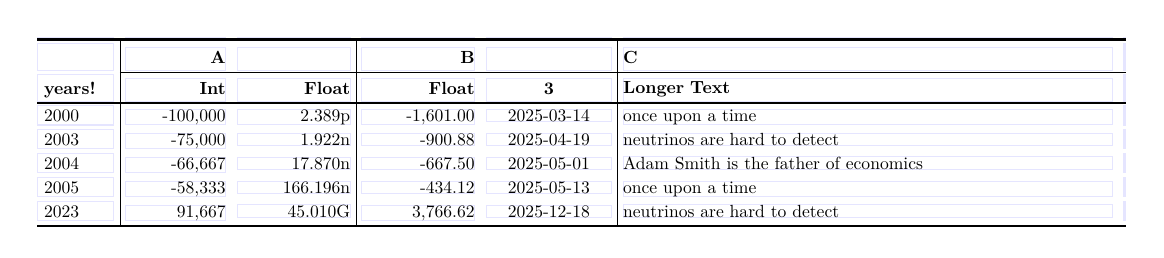
\begin{tikzpicture}[
    auto,
    transform shape,
    nosep/.style={inner sep=0},
    table/.style={
        matrix of nodes,
        row sep=0.125em,
        column sep=0.375em,
        nodes in empty cells,
        nodes={rectangle, scale=0.635, text badly ragged , draw=blue!10},
    row 1/.style={nodes={text=black, anchor=north, inner ysep=0, text height=0, text depth=0}},
    row 2/.style={nodes={text=black, anchor=south, inner ysep=.2em, minimum height=1.3em, font=\bfseries}},
    row 3/.style={nodes={text=black, anchor=south, inner ysep=.2em, minimum height=1.3em, font=\bfseries}},
    column  1/.style={nodes={align=left  }, text height=0.9em, text depth=0.2em, inner xsep=0.375em, inner ysep=0, text width=3.60em},
    column  2/.style={nodes={align=right }, nosep, text width=5.71em},
    column  3/.style={nodes={align=right }, nosep, text width=6.43em},
    column  4/.style={nodes={align=right }, nosep, text width=6.43em},
    column  5/.style={nodes={align=center}, nosep, text width=7.14em},
    column  6/.style={nodes={align=left  }, nosep, text width=27.85em},
    column  7/.style={text height=0.9em, text depth=0.2em, nosep, text width=0em}   }]
\matrix (TGTVSPSJTJM2I) [table, ampersand replacement=\&]{
      \&          \&           \&           \&            \&                                         \& \\
 \grtspacer \& A\grtspacer \& \grtspacer \& B\grtspacer \& \grtspacer \& C\grtspacer                             \& \\
 years!\grtspacer \& Int\grtspacer \& Float\grtspacer \& Float\grtspacer \& 3\grtspacer \& Longer Text\grtspacer                   \& \\
 2000 \& -100,000 \&    2.389p \& -1,601.00 \& 2025-03-14 \& once upon a time                        \& \\
 2003 \&  -75,000 \&    1.922n \&   -900.88 \& 2025-04-19 \&  neutrinos are hard to detect           \& \\
 2004 \&  -66,667 \&   17.870n \&   -667.50 \& 2025-05-01 \&   Adam Smith is the father of economics \& \\
 2005 \&  -58,333 \&  166.196n \&   -434.12 \& 2025-05-13 \& once upon a time                        \& \\
 2023 \&   91,667 \&   45.010G \&  3,766.62 \& 2025-12-18 \&  neutrinos are hard to detect           \& \\
};

\path[draw, thick] (TGTVSPSJTJM2I-1-1.south west)  -- (TGTVSPSJTJM2I-1-7.south east);
\path[draw, semithick] ([yshift=-0.0625em]TGTVSPSJTJM2I-3-1.south west)  -- ([yshift=-0.0625em]TGTVSPSJTJM2I-3-7.south east);
\path[draw, thick] ([yshift=-0.3125em]TGTVSPSJTJM2I-8-1.base west)  -- ([yshift=-0.3125em]TGTVSPSJTJM2I-8-7.base east);
\path[draw, very thin] ([xshift=-0.1875em, yshift=-0.0625em]TGTVSPSJTJM2I-2-2.south west)  -- ([yshift=-0.0625em]TGTVSPSJTJM2I-2-7.south east);
\path[draw, very thin] ([xshift=-0.1875em]TGTVSPSJTJM2I-1-2.south west)  -- ([yshift=-0.3125em, xshift=-0.1875em]TGTVSPSJTJM2I-8-2.base west);
\path[draw, ultra thin] ([xshift=0.1875em, yshift=-0.0625em]TGTVSPSJTJM2I-1-3.south east)  -- ([yshift=-0.3125em, xshift=0.1875em]TGTVSPSJTJM2I-8-3.base east);
\path[draw, ultra thin] ([xshift=0.1875em, yshift=-0.0625em]TGTVSPSJTJM2I-1-5.south east)  -- ([yshift=-0.3125em, xshift=0.1875em]TGTVSPSJTJM2I-8-5.base east);



\end{tikzpicture}

\end{table}%

Here is the raw HTML and LaTeX output.

\footnotesize

\phantomsection\label{raw-output}
\begin{Shaded}
\begin{Highlighting}[]
\NormalTok{f }\OperatorTok{=}\NormalTok{ sGT(hard.head(}\DecValTok{4}\NormalTok{), debug}\OperatorTok{=}\VariableTok{True}\NormalTok{)}
\BuiltInTok{print}\NormalTok{(}\StringTok{\textquotesingle{}HTML output}\CharTok{\textbackslash{}n}\StringTok{\textquotesingle{}}\NormalTok{)}
\BuiltInTok{print}\NormalTok{(f.\_repr\_html\_())}

\BuiltInTok{print}\NormalTok{(}\StringTok{\textquotesingle{}}\CharTok{\textbackslash{}n\textbackslash{}n\textbackslash{}n}\StringTok{TeX output}\CharTok{\textbackslash{}n}\StringTok{\textquotesingle{}}\NormalTok{)}
\BuiltInTok{print}\NormalTok{(f.\_repr\_latex\_())}
\end{Highlighting}
\end{Shaded}

\begin{verbatim}
HTML output

<div class="greater-table">
<style>
    #T6JW65HYNG3A5  {
    border-collapse: collapse;
    font-family: "Roboto", "Open Sans Condensed", "Arial", 'Segoe UI', sans-serif;
    font-size: 0.9em;
    width: auto;
    border: none;
    overflow: auto;
    margin-left: auto;
    margin-right: auto;
    }
    /* tag formats */
    #T6JW65HYNG3A5 caption {
        padding: 8px 10px 4px 10px;
        font-size: 0.99em;
        text-align: center;
        font-weight: normal;
        caption-side: top;
    }
    #T6JW65HYNG3A5 thead {
        /* top and bottom of header */
        border-top: 1px solid #0ff;
        border-bottom: 1px solid #0ff;
        font-size: 0.99em;
        }
    #T6JW65HYNG3A5 tbody {
        /* bottom of body */
        border-bottom: 1px solid #f0f;
        }
    #T6JW65HYNG3A5 th  {
        vertical-align: bottom;
        padding: 8px 10px 8px 10px;
    }
    #T6JW65HYNG3A5 td {
        /* top, right, bottom left cell padding */
        padding: 4px 10px 4px 10px;
        vertical-align: top;
    }
    /* class overrides */
    #T6JW65HYNG3A5 .grt-hrule-0 {
        border-top: 0px solid #f00;
    }
    #T6JW65HYNG3A5 .grt-hrule-1 {
        border-top: 0px solid #b00;
    }
    #T6JW65HYNG3A5 .grt-hrule-2 {
        border-top: 0px solid #900;
    }
    /* for the header, there if you have v lines you want h lines
       hence use vrule_widths */
    #T6JW65HYNG3A5 .grt-bhrule-0 {
        border-bottom: 1.5px solid #f00;
    }
    #T6JW65HYNG3A5 .grt-bhrule-1 {
        border-bottom: 1px solid #b00;
    }
    #T6JW65HYNG3A5 .grt-vrule-index {
        border-left: 1.5px solid #0f0;
    }
    #T6JW65HYNG3A5 .grt-vrule-0 {
        border-left: 1.5px solid #0f0;
    }
    #T6JW65HYNG3A5 .grt-vrule-1 {
        border-left: 1px solid #0a0;
    }
    #T6JW65HYNG3A5 .grt-vrule-2 {
        border-left: 0.5px solid #090;
    }
    #T6JW65HYNG3A5 .grt-left {
        text-align: left;
    }
    #T6JW65HYNG3A5 .grt-center {
        text-align: center;
    }
    #T6JW65HYNG3A5 .grt-right {
        text-align: right;
        font-variant-numeric: tabular-nums;
    }
    #T6JW65HYNG3A5 .grt-head {
        font-family: "Times New Roman", 'Courier New';
        font-size: 0.99em;
    }
    #T6JW65HYNG3A5 .grt-bold {
        font-weight: bold;
    }
</style>
<table id="T6JW65HYNG3A5">
<caption> (id: T6JW65HYNG3A5)</caption>
<thead>
<tr>
<th class="grt-left"></th>
<th class="grt-center grt-bhrule-0 grt-vrule-index" colspan="2">A</th>
<th class="grt-center grt-bhrule-0 grt-vrule-0" colspan="2">B</th>
<th class="grt-center grt-bhrule-0 grt-vrule-0" colspan="1">C</th>
</tr>
<tr>
<th class="grt-left">years!</th>
<th class="grt-center grt-vrule-index" colspan="1">Int</th>
<th class="grt-center grt-vrule-1" colspan="1">Float</th>
<th class="grt-center grt-vrule-0" colspan="1">Float</th>
<th class="grt-center grt-vrule-1" colspan="1">3</th>
<th class="grt-center grt-vrule-0" colspan="1">Longer Text</th>
</tr>
</thead>
<tbody>
<tr>
<td class="grt-left">2000</td>
<td class="grt-right grt-vrule-index">-100,000</td>
<td class="grt-right grt-vrule-1"> 2.389p</td>
<td class="grt-right grt-vrule-0">-1,601.00</td>
<td class="grt-center grt-vrule-1">2025-03-14</td>
<td class="grt-left grt-vrule-0">once upon a time</td>
</tr>
<tr>
<td class="grt-left grt-hrule-0">2001</td>
<td class="grt-right grt-hrule-0 grt-vrule-index">-91,667</td>
<td class="grt-right grt-hrule-0 grt-vrule-1"> 22.217p</td>
<td class="grt-right grt-hrule-0 grt-vrule-0">-1,367.62</td>
<td class="grt-center grt-hrule-0 grt-vrule-1">2025-03-26</td>
<td class="grt-left grt-hrule-0 grt-vrule-0"> risk is hard to define</td>
</tr>
<tr>
<td class="grt-left grt-hrule-0">2002</td>
<td class="grt-right grt-hrule-0 grt-vrule-index">-83,333</td>
<td class="grt-right grt-hrule-0 grt-vrule-1"> 206.619p</td>
<td class="grt-right grt-hrule-0 grt-vrule-0">-1,134.25</td>
<td class="grt-center grt-hrule-0 grt-vrule-1">2025-04-07</td>
<td class="grt-left grt-hrule-0 grt-vrule-0"> not in Kansas anymore</td>
</tr>
<tr>
<td class="grt-left grt-hrule-0">2003</td>
<td class="grt-right grt-hrule-0 grt-vrule-index">-75,000</td>
<td class="grt-right grt-hrule-0 grt-vrule-1"> 1.922n</td>
<td class="grt-right grt-hrule-0 grt-vrule-0">-900.88</td>
<td class="grt-center grt-hrule-0 grt-vrule-1">2025-04-19</td>
<td class="grt-left grt-hrule-0 grt-vrule-0"> neutrinos are hard to detect</td>
</tr>
</tbody>
</table></div>



TeX output


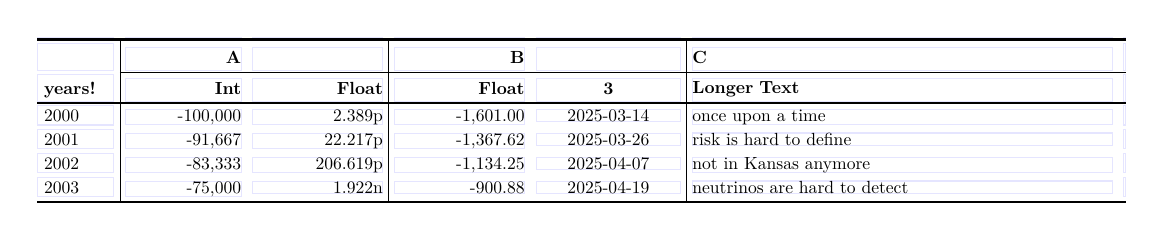
\begin{tikzpicture}[
    auto,
    transform shape,
    nosep/.style={inner sep=0},
    table/.style={
        matrix of nodes,
        row sep=0.125em,
        column sep=0.375em,
        nodes in empty cells,
        nodes={rectangle, scale=0.635, text badly ragged , draw=blue!10},
    row 1/.style={nodes={text=black, anchor=north, inner ysep=0, text height=0, text depth=0}},
    row 2/.style={nodes={text=black, anchor=south, inner ysep=.2em, minimum height=1.3em, font=\bfseries}},
    row 3/.style={nodes={text=black, anchor=south, inner ysep=.2em, minimum height=1.3em, font=\bfseries}},
    column  1/.style={nodes={align=left  }, text height=0.9em, text depth=0.2em, inner xsep=0.375em, inner ysep=0, text width=3.60em},
    column  2/.style={nodes={align=right }, nosep, text width=6.59em},
    column  3/.style={nodes={align=right }, nosep, text width=7.41em},
    column  4/.style={nodes={align=right }, nosep, text width=7.41em},
    column  5/.style={nodes={align=center}, nosep, text width=8.24em},
    column  6/.style={nodes={align=left  }, nosep, text width=23.89em},
    column  7/.style={text height=0.9em, text depth=0.2em, nosep, text width=0em}   }]
\matrix (T6JW65HYNG3A5) [table, ampersand replacement=\&]{
      \&          \&           \&           \&            \&                               \& \\
 \grtspacer \& A\grtspacer \& \grtspacer \& B\grtspacer \& \grtspacer \& C\grtspacer                   \& \\
 years!\grtspacer \& Int\grtspacer \& Float\grtspacer \& Float\grtspacer \& 3\grtspacer \& Longer Text\grtspacer         \& \\
 2000 \& -100,000 \&    2.389p \& -1,601.00 \& 2025-03-14 \& once upon a time              \& \\
 2001 \&  -91,667 \&   22.217p \& -1,367.62 \& 2025-03-26 \&  risk is hard to define       \& \\
 2002 \&  -83,333 \&  206.619p \& -1,134.25 \& 2025-04-07 \&  not in Kansas anymore        \& \\
 2003 \&  -75,000 \&    1.922n \&   -900.88 \& 2025-04-19 \&  neutrinos are hard to detect \& \\
};

\path[draw, thick] (T6JW65HYNG3A5-1-1.south west)  -- (T6JW65HYNG3A5-1-7.south east);
\path[draw, semithick] ([yshift=-0.0625em]T6JW65HYNG3A5-3-1.south west)  -- ([yshift=-0.0625em]T6JW65HYNG3A5-3-7.south east);
\path[draw, thick] ([yshift=-0.3125em]T6JW65HYNG3A5-7-1.base west)  -- ([yshift=-0.3125em]T6JW65HYNG3A5-7-7.base east);
\path[draw, very thin] ([xshift=-0.1875em, yshift=-0.0625em]T6JW65HYNG3A5-2-2.south west)  -- ([yshift=-0.0625em]T6JW65HYNG3A5-2-7.south east);
\path[draw, very thin] ([xshift=-0.1875em]T6JW65HYNG3A5-1-2.south west)  -- ([yshift=-0.3125em, xshift=-0.1875em]T6JW65HYNG3A5-7-2.base west);
\path[draw, ultra thin] ([xshift=0.1875em, yshift=-0.0625em]T6JW65HYNG3A5-1-3.south east)  -- ([yshift=-0.3125em, xshift=0.1875em]T6JW65HYNG3A5-7-3.base east);
\path[draw, ultra thin] ([xshift=0.1875em, yshift=-0.0625em]T6JW65HYNG3A5-1-5.south east)  -- ([yshift=-0.3125em, xshift=0.1875em]T6JW65HYNG3A5-7-5.base east);



\end{tikzpicture}
\end{verbatim}

\normalsize

\section{A Table with TeX Content}\label{a-table-with-tex-content}

\begin{Shaded}
\begin{Highlighting}[]
\NormalTok{index }\OperatorTok{=}\NormalTok{ pd.Index([}\StringTok{"A"}\NormalTok{, }\StringTok{"B"}\NormalTok{, }\StringTok{"$C\_1$"}\NormalTok{, }\StringTok{"C\_2 not tex"}\NormalTok{, }\StringTok{\textquotesingle{}$}\CharTok{\textbackslash{}\textbackslash{}}\StringTok{cos(A)$\textquotesingle{}}\NormalTok{])}
\NormalTok{tex }\OperatorTok{=}\NormalTok{ pd.DataFrame(}
\NormalTok{\{}\StringTok{\textquotesingle{}x\textquotesingle{}}\NormalTok{: np.arange(}\DecValTok{2020}\NormalTok{, }\DecValTok{2025}\NormalTok{, dtype}\OperatorTok{=}\BuiltInTok{int}\NormalTok{),}
\StringTok{\textquotesingle{}b\textquotesingle{}}\NormalTok{: np.random.random(}\DecValTok{5}\NormalTok{),}
\StringTok{\textquotesingle{}a1\textquotesingle{}}\NormalTok{: [}\SpecialStringTok{f\textquotesingle{}$x\^{}}\SpecialCharTok{\{}\NormalTok{i}\SpecialCharTok{\}}\SpecialStringTok{$\textquotesingle{}} \ControlFlowTok{for}\NormalTok{ i }\KeywordTok{in} \BuiltInTok{range}\NormalTok{(}\DecValTok{5}\NormalTok{,}\DecValTok{10}\NormalTok{)],}
\StringTok{\textquotesingle{}a2\textquotesingle{}}\NormalTok{: [}\SpecialStringTok{f\textquotesingle{}$}\CharTok{\textbackslash{}\textbackslash{}}\SpecialStringTok{sin(}\SpecialCharTok{\{}\NormalTok{i}\SpecialCharTok{\}}\SpecialStringTok{x}\CharTok{\textbackslash{}\textbackslash{}}\SpecialStringTok{pi/n)$\textquotesingle{}} \ControlFlowTok{for}\NormalTok{ i }\KeywordTok{in} \BuiltInTok{range}\NormalTok{(}\DecValTok{5}\NormalTok{,}\DecValTok{10}\NormalTok{)],}
\StringTok{\textquotesingle{}a3\textquotesingle{}}\NormalTok{: [}\SpecialStringTok{f\textquotesingle{}$x\^{}}\SpecialCharTok{\{}\NormalTok{i}\SpecialCharTok{\}}\SpecialStringTok{$\textquotesingle{}} \ControlFlowTok{for}\NormalTok{ i }\KeywordTok{in} \BuiltInTok{range}\NormalTok{(}\DecValTok{5}\NormalTok{,}\DecValTok{10}\NormalTok{)],}
\StringTok{\textquotesingle{}a4\textquotesingle{}}\NormalTok{: [}\SpecialStringTok{f\textquotesingle{}}\CharTok{\textbackslash{}\textbackslash{}}\SpecialStringTok{(x\^{}}\SpecialCharTok{\{}\NormalTok{i}\SpecialCharTok{\}}\CharTok{\textbackslash{}\textbackslash{}}\SpecialStringTok{)\textquotesingle{}} \ControlFlowTok{for}\NormalTok{ i }\KeywordTok{in} \BuiltInTok{range}\NormalTok{(}\DecValTok{5}\NormalTok{,}\DecValTok{10}\NormalTok{)],}
\NormalTok{\}).set\_index(}\StringTok{\textquotesingle{}x\textquotesingle{}}\NormalTok{)}
\NormalTok{tex }\OperatorTok{=}\NormalTok{ tex.head()}
\NormalTok{tex.columns }\OperatorTok{=}\NormalTok{ index}
\NormalTok{tex}
\end{Highlighting}
\end{Shaded}

\begin{longtable}[]{@{}llllll@{}}

\caption{\label{tbl-tex}(Quarto generated caption): table displayed by
default routine.}

\tabularnewline

\toprule\noalign{}
& A & B & \$C\_1\$ & C\_2 not tex & \$\textbackslash cos(A)\$ \\
x & & & & & \\
\midrule\noalign{}
\endhead
\bottomrule\noalign{}
\endlastfoot
2020 & 0.501120 & \$x\^{}5\$ &
\$\textbackslash sin(5x\textbackslash pi/n)\$ & \$x\^{}5\$ &
\textbackslash(x\^{}5\textbackslash) \\
2021 & 0.337571 & \$x\^{}6\$ &
\$\textbackslash sin(6x\textbackslash pi/n)\$ & \$x\^{}6\$ &
\textbackslash(x\^{}6\textbackslash) \\
2022 & 0.869421 & \$x\^{}7\$ &
\$\textbackslash sin(7x\textbackslash pi/n)\$ & \$x\^{}7\$ &
\textbackslash(x\^{}7\textbackslash) \\
2023 & 0.219699 & \$x\^{}8\$ &
\$\textbackslash sin(8x\textbackslash pi/n)\$ & \$x\^{}8\$ &
\textbackslash(x\^{}8\textbackslash) \\
2024 & 0.861997 & \$x\^{}9\$ &
\$\textbackslash sin(9x\textbackslash pi/n)\$ & \$x\^{}9\$ &
\textbackslash(x\^{}9\textbackslash) \\

\end{longtable}

\begin{Shaded}
\begin{Highlighting}[]
\NormalTok{sGT(tex, }\StringTok{\textquotesingle{}GT Caption\textquotesingle{}}\NormalTok{)}
\end{Highlighting}
\end{Shaded}

\begin{table}

\caption{\label{tbl-tex-2}(Quarto generated caption)}

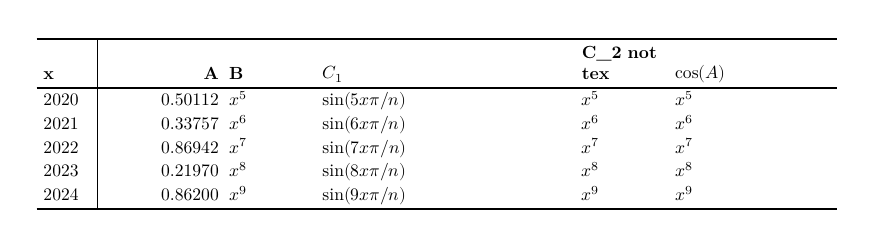
\begin{tikzpicture}[
    auto,
    transform shape,
    nosep/.style={inner sep=0},
    table/.style={
        matrix of nodes,
        row sep=0.125em,
        column sep=0.375em,
        nodes in empty cells,
        nodes={rectangle, scale=0.635, text badly ragged },
    row 1/.style={nodes={text=black, anchor=north, inner ysep=0, text height=0, text depth=0}},
    row 2/.style={nodes={text=black, anchor=south, inner ysep=.2em, minimum height=1.3em, font=\bfseries}},
    column  1/.style={nodes={align=left  }, text height=0.9em, text depth=0.2em, inner xsep=0.375em, inner ysep=0, text width=2.40em},
    column  2/.style={nodes={align=right }, nosep, text width=6.61em},
    column  3/.style={nodes={align=left  }, nosep, text width=4.72em},
    column  4/.style={nodes={align=left  }, nosep, text width=14.17em},
    column  5/.style={nodes={align=left  }, nosep, text width=4.72em},
    column  6/.style={nodes={align=left  }, nosep, text width=8.50em},
    column  7/.style={text height=0.9em, text depth=0.2em, nosep, text width=0em}   }]
\matrix (TCPW6BX3HRZ2T) [table, ampersand replacement=\&]{
      \&         \&       \&                 \&       \&         \& \\
 x\grtspacer \& A\grtspacer \& B\grtspacer \& $C_1$\grtspacer \& C\_2 not tex\grtspacer \& $\cos(A)$\grtspacer \& \\
 2020 \& 0.50112 \& $x^5$ \& $\sin(5x\pi/n)$ \& $x^5$ \& \(x^5\) \& \\
 2021 \& 0.33757 \& $x^6$ \& $\sin(6x\pi/n)$ \& $x^6$ \& \(x^6\) \& \\
 2022 \& 0.86942 \& $x^7$ \& $\sin(7x\pi/n)$ \& $x^7$ \& \(x^7\) \& \\
 2023 \& 0.21970 \& $x^8$ \& $\sin(8x\pi/n)$ \& $x^8$ \& \(x^8\) \& \\
 2024 \& 0.86200 \& $x^9$ \& $\sin(9x\pi/n)$ \& $x^9$ \& \(x^9\) \& \\
};

\path[draw, thick] (TCPW6BX3HRZ2T-1-1.south west)  -- (TCPW6BX3HRZ2T-1-7.south east);
\path[draw, semithick] ([yshift=-0.0625em]TCPW6BX3HRZ2T-2-1.south west)  -- ([yshift=-0.0625em]TCPW6BX3HRZ2T-2-7.south east);
\path[draw, thick] ([yshift=-0.3125em]TCPW6BX3HRZ2T-7-1.base west)  -- ([yshift=-0.3125em]TCPW6BX3HRZ2T-7-7.base east);
\path[draw, very thin] ([xshift=-0.1875em]TCPW6BX3HRZ2T-1-2.south west)  -- ([yshift=-0.3125em, xshift=-0.1875em]TCPW6BX3HRZ2T-7-2.base west);



\end{tikzpicture}

\end{table}%

Ratio columns.

\begin{Shaded}
\begin{Highlighting}[]
\NormalTok{tex.columns }\OperatorTok{=}\NormalTok{ [}\StringTok{"A (\%)"}\NormalTok{, }\StringTok{"B"}\NormalTok{, }\StringTok{"$C\_1$"}\NormalTok{, }\StringTok{"C\_2 not tex"}\NormalTok{, }\StringTok{\textquotesingle{}$}\CharTok{\textbackslash{}\textbackslash{}}\StringTok{cos(A)$\textquotesingle{}}\NormalTok{]}
\NormalTok{sGT(tex, }\StringTok{\textquotesingle{}Ratio columns in A\textquotesingle{}}\NormalTok{, ratio\_cols}\OperatorTok{=}\StringTok{\textquotesingle{}A (\%)\textquotesingle{}}\NormalTok{)}
\end{Highlighting}
\end{Shaded}

\begin{table}

\caption{\label{tbl-tex-3}greater table output}

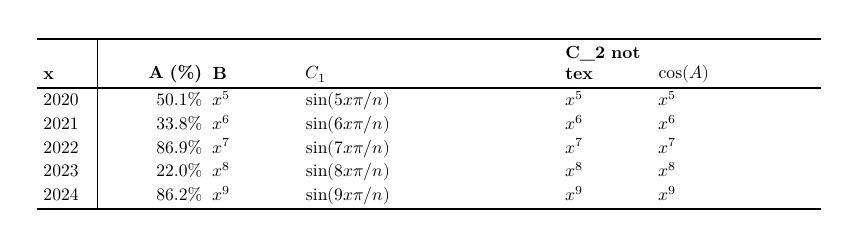
\begin{tikzpicture}[
    auto,
    transform shape,
    nosep/.style={inner sep=0},
    table/.style={
        matrix of nodes,
        row sep=0.125em,
        column sep=0.375em,
        nodes in empty cells,
        nodes={rectangle, scale=0.635, text badly ragged },
    row 1/.style={nodes={text=black, anchor=north, inner ysep=0, text height=0, text depth=0}},
    row 2/.style={nodes={text=black, anchor=south, inner ysep=.2em, minimum height=1.3em, font=\bfseries}},
    column  1/.style={nodes={align=left  }, text height=0.9em, text depth=0.2em, inner xsep=0.375em, inner ysep=0, text width=2.40em},
    column  2/.style={nodes={align=right }, nosep, text width=5.67em},
    column  3/.style={nodes={align=left  }, nosep, text width=4.72em},
    column  4/.style={nodes={align=left  }, nosep, text width=14.17em},
    column  5/.style={nodes={align=left  }, nosep, text width=4.72em},
    column  6/.style={nodes={align=left  }, nosep, text width=8.50em},
    column  7/.style={text height=0.9em, text depth=0.2em, nosep, text width=0em}   }]
\matrix (T5ZEZ3634JGIC) [table, ampersand replacement=\&]{
      \&        \&       \&                 \&       \&         \& \\
 x\grtspacer \& A (\%)\grtspacer \& B\grtspacer \& $C_1$\grtspacer \& C\_2 not tex\grtspacer \& $\cos(A)$\grtspacer \& \\
 2020 \& 50.1\% \& $x^5$ \& $\sin(5x\pi/n)$ \& $x^5$ \& \(x^5\) \& \\
 2021 \& 33.8\% \& $x^6$ \& $\sin(6x\pi/n)$ \& $x^6$ \& \(x^6\) \& \\
 2022 \& 86.9\% \& $x^7$ \& $\sin(7x\pi/n)$ \& $x^7$ \& \(x^7\) \& \\
 2023 \& 22.0\% \& $x^8$ \& $\sin(8x\pi/n)$ \& $x^8$ \& \(x^8\) \& \\
 2024 \& 86.2\% \& $x^9$ \& $\sin(9x\pi/n)$ \& $x^9$ \& \(x^9\) \& \\
};

\path[draw, thick] (T5ZEZ3634JGIC-1-1.south west)  -- (T5ZEZ3634JGIC-1-7.south east);
\path[draw, semithick] ([yshift=-0.0625em]T5ZEZ3634JGIC-2-1.south west)  -- ([yshift=-0.0625em]T5ZEZ3634JGIC-2-7.south east);
\path[draw, thick] ([yshift=-0.3125em]T5ZEZ3634JGIC-7-1.base west)  -- ([yshift=-0.3125em]T5ZEZ3634JGIC-7-7.base east);
\path[draw, very thin] ([xshift=-0.1875em]T5ZEZ3634JGIC-1-2.south west)  -- ([yshift=-0.3125em, xshift=-0.1875em]T5ZEZ3634JGIC-7-2.base west);



\end{tikzpicture}

\end{table}%

\section{Greater\_tables Test Suite}\label{greater_tables-test-suite}

\phantomsection\label{greater-tables-test}
\begin{Shaded}
\begin{Highlighting}[]
\NormalTok{test\_gen }\OperatorTok{=}\NormalTok{ gtu.TestDFGenerator(}\DecValTok{0}\NormalTok{, }\DecValTok{0}\NormalTok{)}
\NormalTok{ans }\OperatorTok{=}\NormalTok{ test\_gen.test\_suite()    }
\end{Highlighting}
\end{Shaded}

\subsection{Test Table: basic}\label{test-table-basic}

\begin{Shaded}
\begin{Highlighting}[]
\NormalTok{hrw }\OperatorTok{=}\NormalTok{ (}\DecValTok{0}\NormalTok{, }\DecValTok{0}\NormalTok{, }\DecValTok{0}\NormalTok{)}
\NormalTok{sGT(ans[}\StringTok{\textquotesingle{}basic\textquotesingle{}}\NormalTok{], }\StringTok{"Basic"}\NormalTok{, ratio\_cols}\OperatorTok{=}\StringTok{\textquotesingle{}z\textquotesingle{}}\NormalTok{, aligners}\OperatorTok{=}\NormalTok{\{}\StringTok{\textquotesingle{}w\textquotesingle{}}\NormalTok{: }\StringTok{\textquotesingle{}l\textquotesingle{}}\NormalTok{\},}
\NormalTok{        hrule\_widths}\OperatorTok{=}\NormalTok{hrw)}
\end{Highlighting}
\end{Shaded}

\begin{table}

\caption{\label{tbl-greater-tables-test-0}GT output for test table
basic}

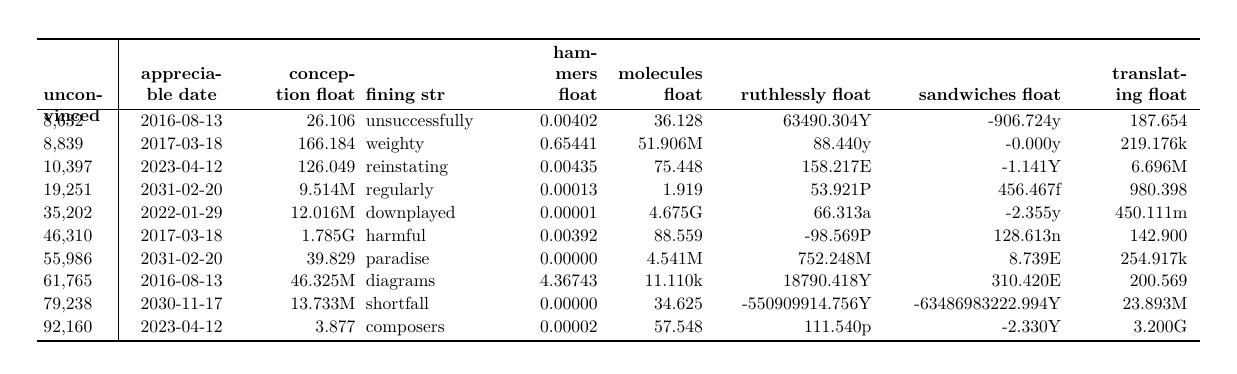
\begin{tikzpicture}[
    auto,
    transform shape,
    nosep/.style={inner sep=0},
    table/.style={
        matrix of nodes,
        row sep=0.125em,
        column sep=0.375em,
        nodes in empty cells,
        nodes={rectangle, scale=0.635, text badly ragged },
    row 1/.style={nodes={text=black, anchor=north, inner ysep=0, text height=0, text depth=0}},
    row 2/.style={nodes={text=black, anchor=south, inner ysep=.2em, minimum height=1.3em, font=\bfseries}},
    column  1/.style={nodes={align=left  }, text height=0.9em, text depth=0.2em, inner xsep=0.375em, inner ysep=0, text width=3.60em},
    column  2/.style={nodes={align=center}, nosep, text width=6.60em},
    column  3/.style={nodes={align=right }, nosep, text width=6.00em},
    column  4/.style={nodes={align=left  }, nosep, text width=8.40em},
    column  5/.style={nodes={align=right }, nosep, text width=4.20em},
    column  6/.style={nodes={align=right }, nosep, text width=5.40em},
    column  7/.style={nodes={align=right }, nosep, text width=9.00em},
    column  8/.style={nodes={align=right }, nosep, text width=10.20em},
    column  9/.style={nodes={align=right }, nosep, text width=6.60em},
    column 10/.style={text height=0.9em, text depth=0.2em, nosep, text width=0em}   }]
\matrix (TGBVQTD6WMYO4) [table, ampersand replacement=\&]{
        \&            \&          \&                \&         \&          \&                 \&                   \&           \& \\
 unconvinced\grtspacer \& appreciable date\grtspacer \& conception float\grtspacer \& fining str\grtspacer \& hammers float\grtspacer \& molecules float\grtspacer \& ruthlessly float\grtspacer \& sandwiches float\grtspacer \& translating float\grtspacer \& \\
 8,632  \& 2016-08-13 \&   26.106 \& unsuccessfully \& 0.00402 \&   36.128 \&      63490.304Y \&         -906.724y \&   187.654 \& \\
 8,839  \& 2017-03-18 \&  166.184 \& weighty        \& 0.65441 \&  51.906M \&         88.440y \&           -0.000y \&  219.176k \& \\
 10,397 \& 2023-04-12 \&  126.049 \& reinstating    \& 0.00435 \&   75.448 \&        158.217E \&           -1.141Y \&    6.696M \& \\
 19,251 \& 2031-02-20 \&   9.514M \& regularly      \& 0.00013 \&    1.919 \&         53.921P \&          456.467f \&   980.398 \& \\
 35,202 \& 2022-01-29 \&  12.016M \& downplayed     \& 0.00001 \&   4.675G \&         66.313a \&           -2.355y \&  450.111m \& \\
 46,310 \& 2017-03-18 \&   1.785G \& harmful        \& 0.00392 \&   88.559 \&        -98.569P \&          128.613n \&   142.900 \& \\
 55,986 \& 2031-02-20 \&   39.829 \& paradise       \& 0.00000 \&   4.541M \&        752.248M \&            8.739E \&  254.917k \& \\
 61,765 \& 2016-08-13 \&  46.325M \& diagrams       \& 4.36743 \&  11.110k \&      18790.418Y \&          310.420E \&   200.569 \& \\
 79,238 \& 2030-11-17 \&  13.733M \& shortfall      \& 0.00000 \&   34.625 \& -550909914.756Y \& -63486983222.994Y \&   23.893M \& \\
 92,160 \& 2023-04-12 \&    3.877 \& composers      \& 0.00002 \&   57.548 \&        111.540p \&           -2.330Y \&    3.200G \& \\
};

\path[draw, thick] (TGBVQTD6WMYO4-1-1.south west)  -- (TGBVQTD6WMYO4-1-10.south east);
\path[draw, semithick] ([yshift=-0.0625em]TGBVQTD6WMYO4-2-1.south west)  -- ([yshift=-0.0625em]TGBVQTD6WMYO4-2-10.south east);
\path[draw, thick] ([yshift=-0.3125em]TGBVQTD6WMYO4-12-1.base west)  -- ([yshift=-0.3125em]TGBVQTD6WMYO4-12-10.base east);
\path[draw, very thin] ([xshift=-0.1875em]TGBVQTD6WMYO4-1-2.south west)  -- ([yshift=-0.3125em, xshift=-0.1875em]TGBVQTD6WMYO4-12-2.base west);



\end{tikzpicture}

\end{table}%

Comments go here.

\subsection{Test Table: timeseries}\label{test-table-timeseries}

\begin{Shaded}
\begin{Highlighting}[]
\NormalTok{hrw }\OperatorTok{=}\NormalTok{ (}\DecValTok{0}\NormalTok{, }\DecValTok{0}\NormalTok{, }\DecValTok{0}\NormalTok{)}
\NormalTok{sGT(ans[}\StringTok{\textquotesingle{}timeseries\textquotesingle{}}\NormalTok{], }\StringTok{"Timeseries"}\NormalTok{, ratio\_cols}\OperatorTok{=}\StringTok{\textquotesingle{}z\textquotesingle{}}\NormalTok{, aligners}\OperatorTok{=}\NormalTok{\{}\StringTok{\textquotesingle{}w\textquotesingle{}}\NormalTok{: }\StringTok{\textquotesingle{}l\textquotesingle{}}\NormalTok{\},}
\NormalTok{        hrule\_widths}\OperatorTok{=}\NormalTok{hrw)}
\end{Highlighting}
\end{Shaded}

\begin{table}

\caption{\label{tbl-greater-tables-test-1}GT output for test table
timeseries}

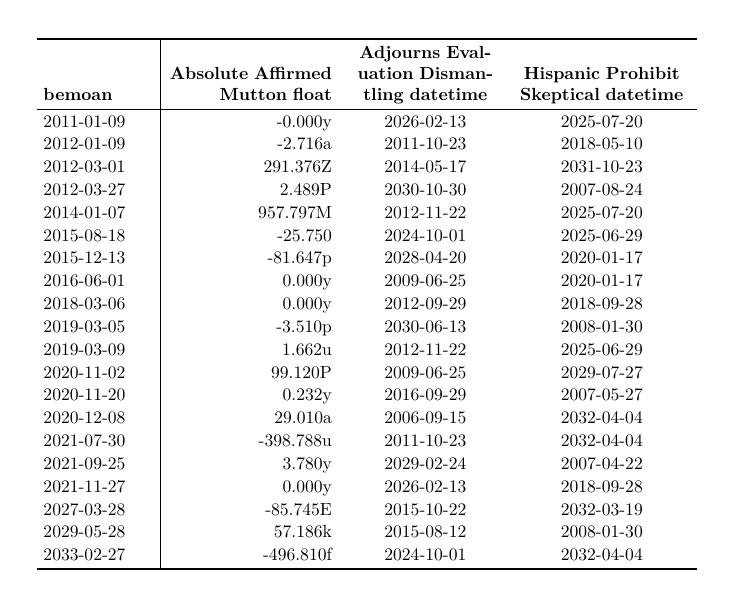
\begin{tikzpicture}[
    auto,
    transform shape,
    nosep/.style={inner sep=0},
    table/.style={
        matrix of nodes,
        row sep=0.125em,
        column sep=0.375em,
        nodes in empty cells,
        nodes={rectangle, scale=0.635, text badly ragged },
    row 1/.style={nodes={text=black, anchor=north, inner ysep=0, text height=0, text depth=0}},
    row 2/.style={nodes={text=black, anchor=south, inner ysep=.2em, minimum height=1.3em, font=\bfseries}},
    column  1/.style={nodes={align=left  }, text height=0.9em, text depth=0.2em, inner xsep=0.375em, inner ysep=0, text width=6.00em},
    column  2/.style={nodes={align=right }, nosep, text width=9.45em},
    column  3/.style={nodes={align=center}, nosep, text width=9.45em},
    column  4/.style={nodes={align=center}, nosep, text width=9.45em},
    column  5/.style={text height=0.9em, text depth=0.2em, nosep, text width=0em}   }]
\matrix (TBSYLUFCI4LBB) [table, ampersand replacement=\&]{
            \&           \&            \&            \& \\
 bemoan\grtspacer \& Absolute Affirmed Mutton float\grtspacer \& Adjourns Evaluation Dismantling datetime\grtspacer \& Hispanic Prohibit Skeptical datetime\grtspacer \& \\
 2011-01-09 \&   -0.000y \& 2026-02-13 \& 2025-07-20 \& \\
 2012-01-09 \&   -2.716a \& 2011-10-23 \& 2018-05-10 \& \\
 2012-03-01 \&  291.376Z \& 2014-05-17 \& 2031-10-23 \& \\
 2012-03-27 \&    2.489P \& 2030-10-30 \& 2007-08-24 \& \\
 2014-01-07 \&  957.797M \& 2012-11-22 \& 2025-07-20 \& \\
 2015-08-18 \&   -25.750 \& 2024-10-01 \& 2025-06-29 \& \\
 2015-12-13 \&  -81.647p \& 2028-04-20 \& 2020-01-17 \& \\
 2016-06-01 \&    0.000y \& 2009-06-25 \& 2020-01-17 \& \\
 2018-03-06 \&    0.000y \& 2012-09-29 \& 2018-09-28 \& \\
 2019-03-05 \&   -3.510p \& 2030-06-13 \& 2008-01-30 \& \\
 2019-03-09 \&    1.662u \& 2012-11-22 \& 2025-06-29 \& \\
 2020-11-02 \&   99.120P \& 2009-06-25 \& 2029-07-27 \& \\
 2020-11-20 \&    0.232y \& 2016-09-29 \& 2007-05-27 \& \\
 2020-12-08 \&   29.010a \& 2006-09-15 \& 2032-04-04 \& \\
 2021-07-30 \& -398.788u \& 2011-10-23 \& 2032-04-04 \& \\
 2021-09-25 \&    3.780y \& 2029-02-24 \& 2007-04-22 \& \\
 2021-11-27 \&    0.000y \& 2026-02-13 \& 2018-09-28 \& \\
 2027-03-28 \&  -85.745E \& 2015-10-22 \& 2032-03-19 \& \\
 2029-05-28 \&   57.186k \& 2015-08-12 \& 2008-01-30 \& \\
 2033-02-27 \& -496.810f \& 2024-10-01 \& 2032-04-04 \& \\
};

\path[draw, thick] (TBSYLUFCI4LBB-1-1.south west)  -- (TBSYLUFCI4LBB-1-5.south east);
\path[draw, semithick] ([yshift=-0.0625em]TBSYLUFCI4LBB-2-1.south west)  -- ([yshift=-0.0625em]TBSYLUFCI4LBB-2-5.south east);
\path[draw, thick] ([yshift=-0.3125em]TBSYLUFCI4LBB-22-1.base west)  -- ([yshift=-0.3125em]TBSYLUFCI4LBB-22-5.base east);
\path[draw, very thin] ([xshift=-0.1875em]TBSYLUFCI4LBB-1-2.south west)  -- ([yshift=-0.3125em, xshift=-0.1875em]TBSYLUFCI4LBB-22-2.base west);



\end{tikzpicture}

\end{table}%

Comments go here.

\subsection{Test Table: multiindex}\label{test-table-multiindex}

\begin{Shaded}
\begin{Highlighting}[]
\NormalTok{hrw }\OperatorTok{=}\NormalTok{ (}\FloatTok{1.5}\NormalTok{, }\FloatTok{1.0}\NormalTok{, }\FloatTok{0.5}\NormalTok{)}
\NormalTok{sGT(ans[}\StringTok{\textquotesingle{}multiindex\textquotesingle{}}\NormalTok{], }\StringTok{"Multiindex"}\NormalTok{, ratio\_cols}\OperatorTok{=}\StringTok{\textquotesingle{}z\textquotesingle{}}\NormalTok{, aligners}\OperatorTok{=}\NormalTok{\{}\StringTok{\textquotesingle{}w\textquotesingle{}}\NormalTok{: }\StringTok{\textquotesingle{}l\textquotesingle{}}\NormalTok{\},}
\NormalTok{        hrule\_widths}\OperatorTok{=}\NormalTok{hrw)}
\end{Highlighting}
\end{Shaded}

\begin{table}

\caption{\label{tbl-greater-tables-test-2}GT output for test table
multiindex}

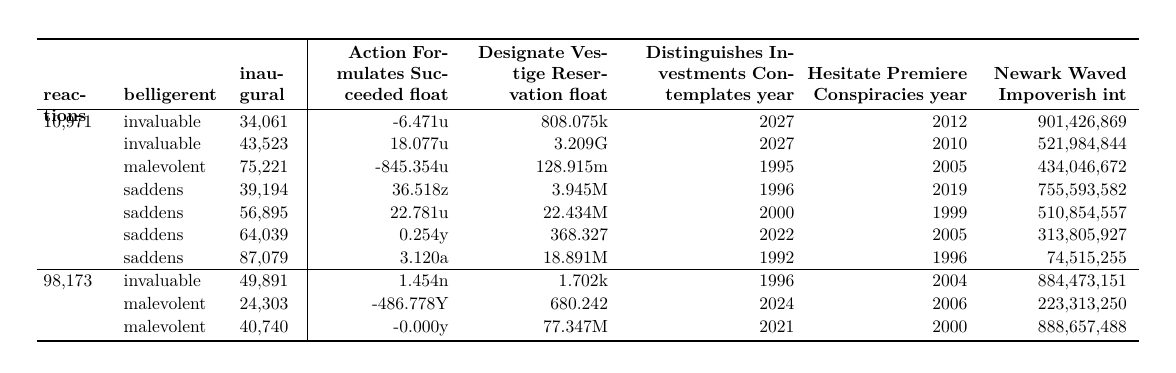
\begin{tikzpicture}[
    auto,
    transform shape,
    nosep/.style={inner sep=0},
    table/.style={
        matrix of nodes,
        row sep=0.125em,
        column sep=0.375em,
        nodes in empty cells,
        nodes={rectangle, scale=0.635, text badly ragged },
    row 1/.style={nodes={text=black, anchor=north, inner ysep=0, text height=0, text depth=0}},
    row 2/.style={nodes={text=black, anchor=south, inner ysep=.2em, minimum height=1.3em, font=\bfseries}},
    column  1/.style={nodes={align=left  }, text height=0.9em, text depth=0.2em, inner xsep=0.375em, inner ysep=0, text width=3.60em},
    column  2/.style={nodes={align=left  }, nosep, text width=6.00em},
    column  3/.style={nodes={align=left  }, nosep, text width=3.60em},
    column  4/.style={nodes={align=right }, nosep, text width=7.71em},
    column  5/.style={nodes={align=right }, nosep, text width=8.48em},
    column  6/.style={nodes={align=right }, nosep, text width=10.02em},
    column  7/.style={nodes={align=right }, nosep, text width=9.25em},
    column  8/.style={nodes={align=right }, nosep, text width=8.48em},
    column  9/.style={text height=0.9em, text depth=0.2em, nosep, text width=0em}   }]
\matrix (TPDCP6TYBOZMN) [table, ampersand replacement=\&]{
        \&            \&        \&           \&           \&      \&      \&             \& \\
 reactions\grtspacer \& belligerent\grtspacer \& inaugural\grtspacer \& Action Formulates Succeeded float\grtspacer \& Designate Vestige Reservation float\grtspacer \& Distinguishes Investments Contemplates year\grtspacer \& Hesitate Premiere Conspiracies year\grtspacer \& Newark Waved Impoverish int\grtspacer \& \\
 10,971 \& invaluable \& 34,061 \&   -6.471u \&  808.075k \& 2027 \& 2012 \& 901,426,869 \& \\
        \& invaluable \& 43,523 \&   18.077u \&    3.209G \& 2027 \& 2010 \& 521,984,844 \& \\
        \& malevolent \& 75,221 \& -845.354u \&  128.915m \& 1995 \& 2005 \& 434,046,672 \& \\
        \& saddens    \& 39,194 \&   36.518z \&    3.945M \& 1996 \& 2019 \& 755,593,582 \& \\
        \& saddens    \& 56,895 \&   22.781u \&   22.434M \& 2000 \& 1999 \& 510,854,557 \& \\
        \& saddens    \& 64,039 \&    0.254y \&   368.327 \& 2022 \& 2005 \& 313,805,927 \& \\
        \& saddens    \& 87,079 \&    3.120a \&   18.891M \& 1992 \& 1996 \&  74,515,255 \& \\
 98,173 \& invaluable \& 49,891 \&    1.454n \&    1.702k \& 1996 \& 2004 \& 884,473,151 \& \\
        \& malevolent \& 24,303 \& -486.778Y \&   680.242 \& 2024 \& 2006 \& 223,313,250 \& \\
        \& malevolent \& 40,740 \&   -0.000y \&   77.347M \& 2021 \& 2000 \& 888,657,488 \& \\
};

\path[draw, thick] (TPDCP6TYBOZMN-1-1.south west)  -- (TPDCP6TYBOZMN-1-9.south east);
\path[draw, very thin] ([yshift=-0.0625em]TPDCP6TYBOZMN-9-1.south west)  -- ([yshift=-0.0625em]TPDCP6TYBOZMN-9-9.south east);
\path[draw, semithick] ([yshift=-0.0625em]TPDCP6TYBOZMN-2-1.south west)  -- ([yshift=-0.0625em]TPDCP6TYBOZMN-2-9.south east);
\path[draw, thick] ([yshift=-0.3125em]TPDCP6TYBOZMN-12-1.base west)  -- ([yshift=-0.3125em]TPDCP6TYBOZMN-12-9.base east);
\path[draw, very thin] ([xshift=-0.1875em]TPDCP6TYBOZMN-1-4.south west)  -- ([yshift=-0.3125em, xshift=-0.1875em]TPDCP6TYBOZMN-12-4.base west);



\end{tikzpicture}

\end{table}%

Comments go here.

\subsection{Test Table: multicolumns}\label{test-table-multicolumns}

\begin{Shaded}
\begin{Highlighting}[]
\NormalTok{hrw }\OperatorTok{=}\NormalTok{ (}\DecValTok{0}\NormalTok{, }\DecValTok{0}\NormalTok{, }\DecValTok{0}\NormalTok{)}
\NormalTok{sGT(ans[}\StringTok{\textquotesingle{}multicolumns\textquotesingle{}}\NormalTok{], }\StringTok{"Multicolumns"}\NormalTok{, ratio\_cols}\OperatorTok{=}\StringTok{\textquotesingle{}z\textquotesingle{}}\NormalTok{, aligners}\OperatorTok{=}\NormalTok{\{}\StringTok{\textquotesingle{}w\textquotesingle{}}\NormalTok{: }\StringTok{\textquotesingle{}l\textquotesingle{}}\NormalTok{\},}
\NormalTok{        hrule\_widths}\OperatorTok{=}\NormalTok{hrw)}
\end{Highlighting}
\end{Shaded}

\begin{table}

\caption{\label{tbl-greater-tables-test-3}GT output for test table
multicolumns}

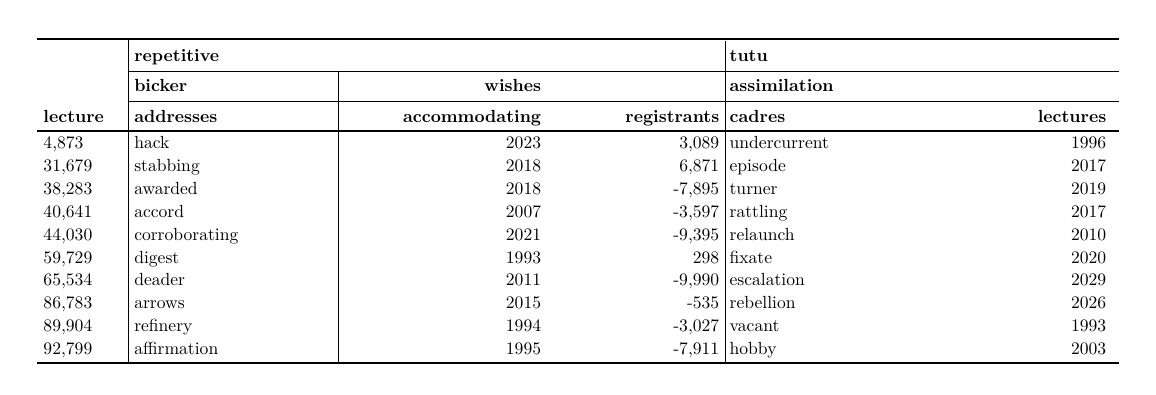
\begin{tikzpicture}[
    auto,
    transform shape,
    nosep/.style={inner sep=0},
    table/.style={
        matrix of nodes,
        row sep=0.125em,
        column sep=0.375em,
        nodes in empty cells,
        nodes={rectangle, scale=0.635, text badly ragged },
    row 1/.style={nodes={text=black, anchor=north, inner ysep=0, text height=0, text depth=0}},
    row 2/.style={nodes={text=black, anchor=south, inner ysep=.2em, minimum height=1.3em, font=\bfseries}},
    row 3/.style={nodes={text=black, anchor=south, inner ysep=.2em, minimum height=1.3em, font=\bfseries}},
    row 4/.style={nodes={text=black, anchor=south, inner ysep=.2em, minimum height=1.3em, font=\bfseries}},
    column  1/.style={nodes={align=left  }, text height=0.9em, text depth=0.2em, inner xsep=0.375em, inner ysep=0, text width=4.20em},
    column  2/.style={nodes={align=left  }, nosep, text width=11.28em},
    column  3/.style={nodes={align=right }, nosep, text width=11.28em},
    column  4/.style={nodes={align=right }, nosep, text width=9.55em},
    column  5/.style={nodes={align=left  }, nosep, text width=10.42em},
    column  6/.style={nodes={align=right }, nosep, text width=10.42em},
    column  7/.style={text height=0.9em, text depth=0.2em, nosep, text width=0em}   }]
\matrix (TNTJBCNKN57RB) [table, ampersand replacement=\&]{
        \&               \&      \&        \&              \&      \& \\
 \grtspacer \& repetitive\grtspacer \& \grtspacer \& \grtspacer \& tutu\grtspacer \& \grtspacer \& \\
 \grtspacer \& bicker\grtspacer \& wishes\grtspacer \& \grtspacer \& assimilation\grtspacer \& \grtspacer \& \\
 lecture\grtspacer \& addresses\grtspacer \& accommodating\grtspacer \& registrants\grtspacer \& cadres\grtspacer \& lectures\grtspacer \& \\
 4,873  \& hack          \& 2023 \&  3,089 \& undercurrent \& 1996 \& \\
 31,679 \& stabbing      \& 2018 \&  6,871 \& episode      \& 2017 \& \\
 38,283 \& awarded       \& 2018 \& -7,895 \& turner       \& 2019 \& \\
 40,641 \& accord        \& 2007 \& -3,597 \& rattling     \& 2017 \& \\
 44,030 \& corroborating \& 2021 \& -9,395 \& relaunch     \& 2010 \& \\
 59,729 \& digest        \& 1993 \&    298 \& fixate       \& 2020 \& \\
 65,534 \& deader        \& 2011 \& -9,990 \& escalation   \& 2029 \& \\
 86,783 \& arrows        \& 2015 \&   -535 \& rebellion    \& 2026 \& \\
 89,904 \& refinery      \& 1994 \& -3,027 \& vacant       \& 1993 \& \\
 92,799 \& affirmation   \& 1995 \& -7,911 \& hobby        \& 2003 \& \\
};

\path[draw, thick] (TNTJBCNKN57RB-1-1.south west)  -- (TNTJBCNKN57RB-1-7.south east);
\path[draw, semithick] ([yshift=-0.0625em]TNTJBCNKN57RB-4-1.south west)  -- ([yshift=-0.0625em]TNTJBCNKN57RB-4-7.south east);
\path[draw, thick] ([yshift=-0.3125em]TNTJBCNKN57RB-14-1.base west)  -- ([yshift=-0.3125em]TNTJBCNKN57RB-14-7.base east);
\path[draw, very thin] ([xshift=-0.1875em, yshift=-0.0625em]TNTJBCNKN57RB-2-2.south west)  -- ([yshift=-0.0625em]TNTJBCNKN57RB-2-7.south east);
\path[draw, very thin] ([xshift=-0.1875em, yshift=-0.0625em]TNTJBCNKN57RB-3-2.south west)  -- ([yshift=-0.0625em]TNTJBCNKN57RB-3-7.south east);
\path[draw, very thin] ([xshift=-0.1875em]TNTJBCNKN57RB-1-2.south west)  -- ([yshift=-0.3125em, xshift=-0.1875em]TNTJBCNKN57RB-14-2.base west);
\path[draw, ultra thin] ([xshift=0.1875em, yshift=-0.0625em]TNTJBCNKN57RB-1-4.south east)  -- ([yshift=-0.3125em, xshift=0.1875em]TNTJBCNKN57RB-14-4.base east);
\path[draw, ultra thin] ([xshift=0.1875em, yshift=-0.0625em]TNTJBCNKN57RB-2-2.south east)  -- ([yshift=-0.3125em, xshift=0.1875em]TNTJBCNKN57RB-14-2.base east);



\end{tikzpicture}

\end{table}%

Comments go here.

\subsection{Test Table: complex}\label{test-table-complex}

\begin{Shaded}
\begin{Highlighting}[]
\NormalTok{hrw }\OperatorTok{=}\NormalTok{ (}\FloatTok{1.5}\NormalTok{, }\FloatTok{1.0}\NormalTok{, }\FloatTok{0.5}\NormalTok{)}
\NormalTok{sGT(ans[}\StringTok{\textquotesingle{}complex\textquotesingle{}}\NormalTok{], }\StringTok{"Complex"}\NormalTok{, ratio\_cols}\OperatorTok{=}\StringTok{\textquotesingle{}z\textquotesingle{}}\NormalTok{, aligners}\OperatorTok{=}\NormalTok{\{}\StringTok{\textquotesingle{}w\textquotesingle{}}\NormalTok{: }\StringTok{\textquotesingle{}l\textquotesingle{}}\NormalTok{\},}
\NormalTok{        hrule\_widths}\OperatorTok{=}\NormalTok{hrw)}
\end{Highlighting}
\end{Shaded}

\begin{table}

\caption{\label{tbl-greater-tables-test-4}GT output for test table
complex}

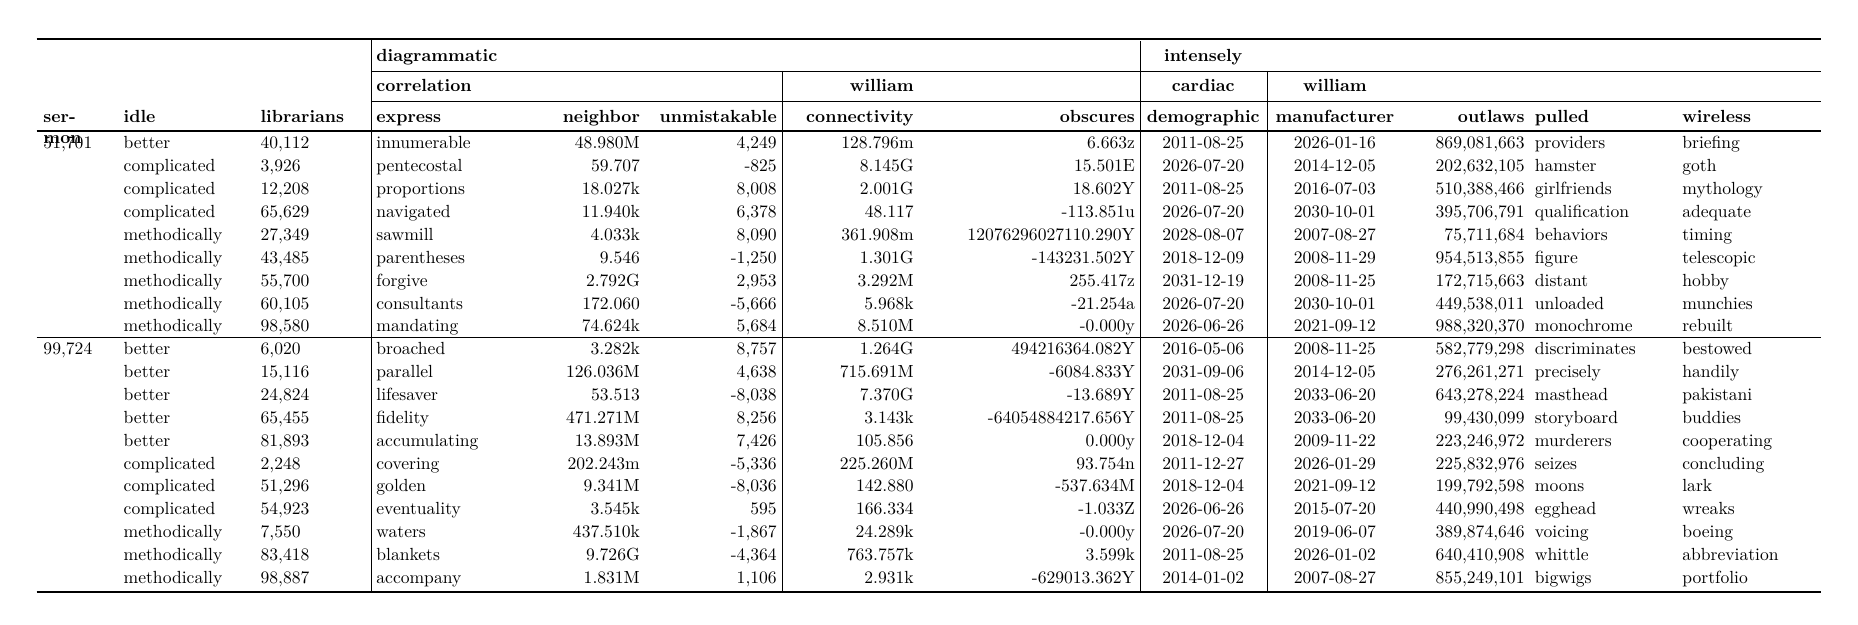
\begin{tikzpicture}[
    auto,
    transform shape,
    nosep/.style={inner sep=0},
    table/.style={
        matrix of nodes,
        row sep=0.125em,
        column sep=0.375em,
        nodes in empty cells,
        nodes={rectangle, scale=0.635, text badly ragged },
    row 1/.style={nodes={text=black, anchor=north, inner ysep=0, text height=0, text depth=0}},
    row 2/.style={nodes={text=black, anchor=south, inner ysep=.2em, minimum height=1.3em, font=\bfseries}},
    row 3/.style={nodes={text=black, anchor=south, inner ysep=.2em, minimum height=1.3em, font=\bfseries}},
    row 4/.style={nodes={text=black, anchor=south, inner ysep=.2em, minimum height=1.3em, font=\bfseries}},
    column  1/.style={nodes={align=left  }, text height=0.9em, text depth=0.2em, inner xsep=0.375em, inner ysep=0, text width=3.60em},
    column  2/.style={nodes={align=left  }, nosep, text width=7.20em},
    column  3/.style={nodes={align=left  }, nosep, text width=6.00em},
    column  4/.style={nodes={align=left  }, nosep, text width=7.20em},
    column  5/.style={nodes={align=right }, nosep, text width=7.20em},
    column  6/.style={nodes={align=right }, nosep, text width=7.20em},
    column  7/.style={nodes={align=right }, nosep, text width=7.20em},
    column  8/.style={nodes={align=right }, nosep, text width=12.00em},
    column  9/.style={nodes={align=center}, nosep, text width=6.60em},
    column 10/.style={nodes={align=center}, nosep, text width=7.20em},
    column 11/.style={nodes={align=right }, nosep, text width=6.60em},
    column 12/.style={nodes={align=left  }, nosep, text width=7.80em},
    column 13/.style={nodes={align=left  }, nosep, text width=7.20em},
    column 14/.style={text height=0.9em, text depth=0.2em, nosep, text width=0em}   }]
\matrix (TYKTNDZBEDOSG) [table, ampersand replacement=\&]{
        \&              \&        \&              \&           \&        \&           \&                      \&            \&            \&             \&               \&              \& \\
 \grtspacer \& \grtspacer   \& \grtspacer \& diagrammatic\grtspacer \& \grtspacer \& \grtspacer \& \grtspacer \&           \grtspacer \& intensely\grtspacer \& \grtspacer \&  \grtspacer \& \grtspacer    \& \grtspacer   \& \\
 \grtspacer \& \grtspacer   \& \grtspacer \& correlation\grtspacer \& \grtspacer \& \grtspacer \& william\grtspacer \&           \grtspacer \& cardiac\grtspacer \& william\grtspacer \&  \grtspacer \& \grtspacer    \& \grtspacer   \& \\
 sermon\grtspacer \& idle\grtspacer \& librarians\grtspacer \& express\grtspacer \& neighbor\grtspacer \& unmistakable\grtspacer \& connectivity\grtspacer \&   obscures\grtspacer \& demographic\grtspacer \& manufacturer\grtspacer \& outlaws\grtspacer \& pulled\grtspacer \& wireless\grtspacer \& \\
 51,701 \& better       \& 40,112 \& innumerable  \&   48.980M \&  4,249 \&  128.796m \&               6.663z \& 2011-08-25 \& 2026-01-16 \& 869,081,663 \& providers     \& briefing     \& \\
        \& complicated  \& 3,926  \& pentecostal  \&    59.707 \&   -825 \&    8.145G \&              15.501E \& 2026-07-20 \& 2014-12-05 \& 202,632,105 \& hamster       \& goth         \& \\
        \& complicated  \& 12,208 \& proportions  \&   18.027k \&  8,008 \&    2.001G \&              18.602Y \& 2011-08-25 \& 2016-07-03 \& 510,388,466 \& girlfriends   \& mythology    \& \\
        \& complicated  \& 65,629 \& navigated    \&   11.940k \&  6,378 \&    48.117 \&            -113.851u \& 2026-07-20 \& 2030-10-01 \& 395,706,791 \& qualification \& adequate     \& \\
        \& methodically \& 27,349 \& sawmill      \&    4.033k \&  8,090 \&  361.908m \&  12076296027110.290Y \& 2028-08-07 \& 2007-08-27 \&  75,711,684 \& behaviors     \& timing       \& \\
        \& methodically \& 43,485 \& parentheses  \&     9.546 \& -1,250 \&    1.301G \&         -143231.502Y \& 2018-12-09 \& 2008-11-29 \& 954,513,855 \& figure        \& telescopic   \& \\
        \& methodically \& 55,700 \& forgive      \&    2.792G \&  2,953 \&    3.292M \&             255.417z \& 2031-12-19 \& 2008-11-25 \& 172,715,663 \& distant       \& hobby        \& \\
        \& methodically \& 60,105 \& consultants  \&   172.060 \& -5,666 \&    5.968k \&             -21.254a \& 2026-07-20 \& 2030-10-01 \& 449,538,011 \& unloaded      \& munchies     \& \\
        \& methodically \& 98,580 \& mandating    \&   74.624k \&  5,684 \&    8.510M \&              -0.000y \& 2026-06-26 \& 2021-09-12 \& 988,320,370 \& monochrome    \& rebuilt      \& \\
 99,724 \& better       \& 6,020  \& broached     \&    3.282k \&  8,757 \&    1.264G \&       494216364.082Y \& 2016-05-06 \& 2008-11-25 \& 582,779,298 \& discriminates \& bestowed     \& \\
        \& better       \& 15,116 \& parallel     \&  126.036M \&  4,638 \&  715.691M \&           -6084.833Y \& 2031-09-06 \& 2014-12-05 \& 276,261,271 \& precisely     \& handily      \& \\
        \& better       \& 24,824 \& lifesaver    \&    53.513 \& -8,038 \&    7.370G \&             -13.689Y \& 2011-08-25 \& 2033-06-20 \& 643,278,224 \& masthead      \& pakistani    \& \\
        \& better       \& 65,455 \& fidelity     \&  471.271M \&  8,256 \&    3.143k \&    -64054884217.656Y \& 2011-08-25 \& 2033-06-20 \&  99,430,099 \& storyboard    \& buddies      \& \\
        \& better       \& 81,893 \& accumulating \&   13.893M \&  7,426 \&   105.856 \&               0.000y \& 2018-12-04 \& 2009-11-22 \& 223,246,972 \& murderers     \& cooperating  \& \\
        \& complicated  \& 2,248  \& covering     \&  202.243m \& -5,336 \&  225.260M \&              93.754n \& 2011-12-27 \& 2026-01-29 \& 225,832,976 \& seizes        \& concluding   \& \\
        \& complicated  \& 51,296 \& golden       \&    9.341M \& -8,036 \&   142.880 \&            -537.634M \& 2018-12-04 \& 2021-09-12 \& 199,792,598 \& moons         \& lark         \& \\
        \& complicated  \& 54,923 \& eventuality  \&    3.545k \&    595 \&   166.334 \&              -1.033Z \& 2026-06-26 \& 2015-07-20 \& 440,990,498 \& egghead       \& wreaks       \& \\
        \& methodically \& 7,550  \& waters       \&  437.510k \& -1,867 \&   24.289k \&              -0.000y \& 2026-07-20 \& 2019-06-07 \& 389,874,646 \& voicing       \& boeing       \& \\
        \& methodically \& 83,418 \& blankets     \&    9.726G \& -4,364 \&  763.757k \&               3.599k \& 2011-08-25 \& 2026-01-02 \& 640,410,908 \& whittle       \& abbreviation \& \\
        \& methodically \& 98,887 \& accompany    \&    1.831M \&  1,106 \&    2.931k \&         -629013.362Y \& 2014-01-02 \& 2007-08-27 \& 855,249,101 \& bigwigs       \& portfolio    \& \\
};

\path[draw, thick] (TYKTNDZBEDOSG-1-1.south west)  -- (TYKTNDZBEDOSG-1-14.south east);
\path[draw, thick] ([yshift=-0.3125em]TYKTNDZBEDOSG-24-1.base west)  -- ([yshift=-0.3125em]TYKTNDZBEDOSG-24-14.base east);
\path[draw, semithick] ([yshift=-0.0625em]TYKTNDZBEDOSG-4-1.south west)  -- ([yshift=-0.0625em]TYKTNDZBEDOSG-4-14.south east);
\path[draw, very thin] ([yshift=-0.0625em]TYKTNDZBEDOSG-13-1.south west)  -- ([yshift=-0.0625em]TYKTNDZBEDOSG-13-14.south east);
\path[draw, very thin] ([xshift=-0.1875em, yshift=-0.0625em]TYKTNDZBEDOSG-2-4.south west)  -- ([yshift=-0.0625em]TYKTNDZBEDOSG-2-14.south east);
\path[draw, very thin] ([xshift=-0.1875em, yshift=-0.0625em]TYKTNDZBEDOSG-3-4.south west)  -- ([yshift=-0.0625em]TYKTNDZBEDOSG-3-14.south east);
\path[draw, very thin] ([xshift=-0.1875em]TYKTNDZBEDOSG-1-4.south west)  -- ([yshift=-0.3125em, xshift=-0.1875em]TYKTNDZBEDOSG-24-4.base west);
\path[draw, ultra thin] ([xshift=0.1875em, yshift=-0.0625em]TYKTNDZBEDOSG-1-8.south east)  -- ([yshift=-0.3125em, xshift=0.1875em]TYKTNDZBEDOSG-24-8.base east);
\path[draw, ultra thin] ([xshift=0.1875em, yshift=-0.0625em]TYKTNDZBEDOSG-2-6.south east)  -- ([yshift=-0.3125em, xshift=0.1875em]TYKTNDZBEDOSG-24-6.base east);
\path[draw, ultra thin] ([xshift=0.1875em, yshift=-0.0625em]TYKTNDZBEDOSG-2-9.south east)  -- ([yshift=-0.3125em, xshift=0.1875em]TYKTNDZBEDOSG-24-9.base east);



\end{tikzpicture}

\end{table}%

Comments go here.

\section{Other input formats}\label{other-input-formats}

\subsection{Markown}\label{markown}

\begin{longtable}[]{@{}
  >{\raggedright\arraybackslash}p{(\linewidth - 6\tabcolsep) * \real{0.7093}}
  >{\centering\arraybackslash}p{(\linewidth - 6\tabcolsep) * \real{0.1047}}
  >{\centering\arraybackslash}p{(\linewidth - 6\tabcolsep) * \real{0.0930}}
  >{\centering\arraybackslash}p{(\linewidth - 6\tabcolsep) * \real{0.0930}}@{}}
\toprule\noalign{}
\begin{minipage}[b]{\linewidth}\raggedright
\textbf{Insured group or insurance product}
\end{minipage} & \begin{minipage}[b]{\linewidth}\centering
\textbf{Sat}
\end{minipage} & \begin{minipage}[b]{\linewidth}\centering
\textbf{RP}
\end{minipage} & \begin{minipage}[b]{\linewidth}\centering
\textbf{RF}
\end{minipage} \\
\midrule\noalign{}
\endhead
\bottomrule\noalign{}
\endlastfoot
Non-standard auto & x & & \\
General liability for judgment proof corporation & x & & \\
Term life insurance & & x & \\
Catastrophe Reinsurance, outside rating agency bounds & & x & \\
High limit property per risk reinsurance & & x & \\
Personal lines for affluent individuals & x & x & \\
Small commercial lines & x & x & \\
Catastrophe reinsurance, within rating agency bounds & x & x & \\
Large account captive reinsurance & & & x \\
Structured quota share, requiring a risk transfer test & x & & x \\
Working layer casualty excess of loss & & x & x \\
Surplus relief quota share on cat exposed line & x & x & x \\
Middle market commercial lines work comp or commercial auto & x & x &
x \\
\end{longtable}

\begin{Shaded}
\begin{Highlighting}[]
\NormalTok{txt }\OperatorTok{=} \StringTok{\textquotesingle{}\textquotesingle{}\textquotesingle{}}

\StringTok{| **Insured group or insurance product**                      | **Sat** | **RP** | **RF** |}
\StringTok{|:{-}{-}{-}{-}{-}{-}{-}{-}{-}{-}{-}{-}{-}{-}{-}{-}{-}{-}{-}{-}{-}{-}{-}{-}{-}{-}{-}{-}{-}{-}{-}{-}{-}{-}{-}{-}{-}{-}{-}{-}{-}{-}{-}{-}{-}{-}{-}{-}{-}{-}{-}{-}{-}{-}{-}{-}{-}{-}{-}{-}|:{-}{-}{-}{-}{-}{-}{-}:|:{-}{-}{-}{-}{-}{-}:|:{-}{-}{-}{-}{-}{-}:|}
\StringTok{| Non{-}standard auto                                           |    x    |        |        |}
\StringTok{| General liability for judgment proof corporation            |    x    |        |        |}
\StringTok{| Term life insurance                                         |         |   x    |        |}
\StringTok{| Catastrophe Reinsurance, outside rating agency bounds       |         |   x    |        |}
\StringTok{| High limit property per risk reinsurance                    |         |   x    |        |}
\StringTok{| Personal lines for affluent individuals                     |    x    |   x    |        |}
\StringTok{| Small commercial lines                                      |    x    |   x    |        |}
\StringTok{| Catastrophe reinsurance, within rating agency bounds        |    x    |   x    |        |}
\StringTok{| Large account captive reinsurance                           |         |        |   x    |}
\StringTok{| Structured quota share, requiring a risk transfer test      |    x    |        |   x    |}
\StringTok{| Working layer casualty excess of loss                       |         |   x    |   x    |}
\StringTok{| Surplus relief quota share on cat exposed line              |    x    |   x    |   x    |}
\StringTok{| Middle market commercial lines work comp or commercial auto |    x    |   x    |   x    |}


\StringTok{\textquotesingle{}\textquotesingle{}\textquotesingle{}}

\NormalTok{GT(txt)}
\end{Highlighting}
\end{Shaded}

\begin{table}

\caption{\label{tbl-greater-tables-test-5}GT from markdown table input}

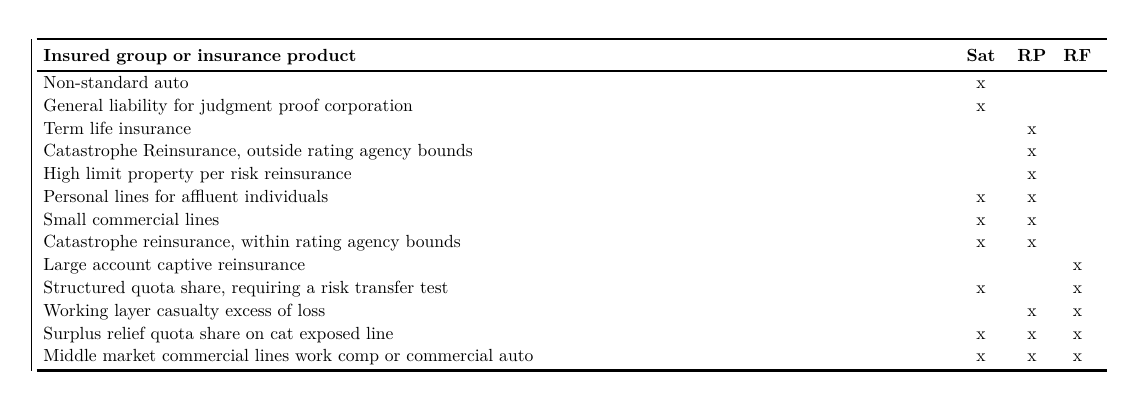
\begin{tikzpicture}[
    auto,
    transform shape,
    nosep/.style={inner sep=0},
    table/.style={
        matrix of nodes,
        row sep=0.125em,
        column sep=0.375em,
        nodes in empty cells,
        nodes={rectangle, scale=0.635, text badly ragged },
    row 1/.style={nodes={text=black, anchor=north, inner ysep=0, text height=0, text depth=0}},
    row 2/.style={nodes={text=black, anchor=south, inner ysep=.2em, minimum height=1.3em, font=\bfseries}},
    column  1/.style={nodes={align=left  }, text height=0.9em, text depth=0.2em, inner xsep=0.375em, inner ysep=0, text width=51.09em},
    column  2/.style={nodes={align=center}, nosep, text width=2.60em},
    column  3/.style={nodes={align=center}, nosep, text width=2.00em},
    column  4/.style={nodes={align=center}, nosep, text width=2.00em},
    column  5/.style={text height=0.9em, text depth=0.2em, nosep, text width=0em}   }]
\matrix (TEQZIBDCCW47A) [table, ampersand replacement=\&]{
                                                             \&   \&   \&   \& \\
 Insured group or insurance product\grtspacer                \& Sat\grtspacer \& RP\grtspacer \& RF\grtspacer \& \\
 Non-standard auto                                           \& x \&   \&   \& \\
 General liability for judgment proof corporation            \& x \&   \&   \& \\
 Term life insurance                                         \&   \& x \&   \& \\
 Catastrophe Reinsurance, outside rating agency bounds       \&   \& x \&   \& \\
 High limit property per risk reinsurance                    \&   \& x \&   \& \\
 Personal lines for affluent individuals                     \& x \& x \&   \& \\
 Small commercial lines                                      \& x \& x \&   \& \\
 Catastrophe reinsurance, within rating agency bounds        \& x \& x \&   \& \\
 Large account captive reinsurance                           \&   \&   \& x \& \\
 Structured quota share, requiring a risk transfer test      \& x \&   \& x \& \\
 Working layer casualty excess of loss                       \&   \& x \& x \& \\
 Surplus relief quota share on cat exposed line              \& x \& x \& x \& \\
 Middle market commercial lines work comp or commercial auto \& x \& x \& x \& \\
};

\path[draw, thick] (TEQZIBDCCW47A-1-1.south west)  -- (TEQZIBDCCW47A-1-5.south east);
\path[draw, semithick] ([yshift=-0.0625em]TEQZIBDCCW47A-2-1.south west)  -- ([yshift=-0.0625em]TEQZIBDCCW47A-2-5.south east);
\path[draw, thick] ([yshift=-0.3125em]TEQZIBDCCW47A-15-1.base west)  -- ([yshift=-0.3125em]TEQZIBDCCW47A-15-5.base east);
\path[draw, very thin] ([xshift=-0.1875em]TEQZIBDCCW47A-1-1.south west)  -- ([yshift=-0.3125em, xshift=-0.1875em]TEQZIBDCCW47A-15-1.base west);



\end{tikzpicture}

\end{table}%

\subsection{List of lists}\label{list-of-lists}

\begin{Shaded}
\begin{Highlighting}[]
\NormalTok{lol }\OperatorTok{=}\NormalTok{ [[}\StringTok{\textquotesingle{}a\textquotesingle{}}\NormalTok{, }\StringTok{\textquotesingle{}b\textquotesingle{}}\NormalTok{, }\StringTok{\textquotesingle{}c\textquotesingle{}}\NormalTok{, }\StringTok{\textquotesingle{}d\textquotesingle{}}\NormalTok{], [}\StringTok{\textquotesingle{}west\textquotesingle{}}\NormalTok{, }\DecValTok{10}\NormalTok{, }\DecValTok{20}\NormalTok{, }\DecValTok{30}\NormalTok{], [}\StringTok{\textquotesingle{}east\textquotesingle{}}\NormalTok{, }\DecValTok{10}\NormalTok{, }\DecValTok{200}\NormalTok{, }\DecValTok{30}\NormalTok{], [}\StringTok{\textquotesingle{}north\textquotesingle{}}\NormalTok{, }\DecValTok{10}\NormalTok{, }\DecValTok{20}\NormalTok{, }\DecValTok{300}\NormalTok{], [}\StringTok{\textquotesingle{}south\textquotesingle{}}\NormalTok{, }\DecValTok{100}\NormalTok{, }\DecValTok{20}\NormalTok{, }\DecValTok{30}\NormalTok{]]}
\NormalTok{GT(lol)}
\end{Highlighting}
\end{Shaded}

\begin{table}

\caption{\label{tbl-greater-tables-test-6}GT output for list of lists
input}

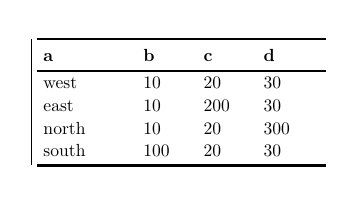
\begin{tikzpicture}[
    auto,
    transform shape,
    nosep/.style={inner sep=0},
    table/.style={
        matrix of nodes,
        row sep=0.125em,
        column sep=0.375em,
        nodes in empty cells,
        nodes={rectangle, scale=0.635, text badly ragged },
    row 1/.style={nodes={text=black, anchor=north, inner ysep=0, text height=0, text depth=0}},
    row 2/.style={nodes={text=black, anchor=south, inner ysep=.2em, minimum height=1.3em, font=\bfseries}},
    column  1/.style={nodes={align=left  }, text height=0.9em, text depth=0.2em, inner xsep=0.375em, inner ysep=0, text width=4.72em},
    column  2/.style={nodes={align=left  }, nosep, text width=2.83em},
    column  3/.style={nodes={align=left  }, nosep, text width=2.83em},
    column  4/.style={nodes={align=left  }, nosep, text width=2.83em},
    column  5/.style={text height=0.9em, text depth=0.2em, nosep, text width=0em}   }]
\matrix (T4XHJ53EN656B) [table, ampersand replacement=\&]{
       \&     \&     \&     \& \\
 a\grtspacer \& b\grtspacer \& c\grtspacer \& d\grtspacer \& \\
 west  \& 10  \& 20  \& 30  \& \\
 east  \& 10  \& 200 \& 30  \& \\
 north \& 10  \& 20  \& 300 \& \\
 south \& 100 \& 20  \& 30  \& \\
};

\path[draw, thick] (T4XHJ53EN656B-1-1.south west)  -- (T4XHJ53EN656B-1-5.south east);
\path[draw, semithick] ([yshift=-0.0625em]T4XHJ53EN656B-2-1.south west)  -- ([yshift=-0.0625em]T4XHJ53EN656B-2-5.south east);
\path[draw, thick] ([yshift=-0.3125em]T4XHJ53EN656B-6-1.base west)  -- ([yshift=-0.3125em]T4XHJ53EN656B-6-5.base east);
\path[draw, very thin] ([xshift=-0.1875em]T4XHJ53EN656B-1-1.south west)  -- ([yshift=-0.3125em, xshift=-0.1875em]T4XHJ53EN656B-6-1.base west);



\end{tikzpicture}

\end{table}%




\end{document}
